% !TeX encoding = UTF-8
\begin{center}
	\begin{minipage}{\textwidth}
		\begin{traditionalpoem}
			از هر کرانه تیر دعا کرده‌ام روان 		  & 
			
			باشد کز آن میانه یکی کارگر شود 	 \\
			
			بس نکته غیر حسن بباید که تا کسی	    	  &
			
			مقبول طبع مردم صاحب نظر شود  \\
			\\
			& 
			\hspace{45pt}
			حافظ
		\end{traditionalpoem}
	\end{minipage}
\end{center}

%------------------------------------------------------------------------------------------------------------%


%$$$$$$$$$$$
%$$$$$$$$$$$
%$$$$$$$$$$$
%$$$$$$  DETECTION  $$$$$$$$$$
%$$$$$$$$$$$
%$$$$$$$$$$$
%$$$$$$$$$$$

%------------------------------------------------------------------------------------------------------------%

\section{طراحی  خط مشی آشکارسازی}
\label{sec:detection}
\par
در فصل‌های گذشته مروری داشتیم بر کیهان‌شناسی نوین، درباره ریسمان‌های کیهانی و ردپایش بر تابش زمینه سخن گفتیم و ابزاری که از علم داده قرض گرفته‌ایم را معرفی کردیم. پس از معرفی داده‌ها و شبیه‌سازی‌های لازم، اکنون آمادگی این را داریم که به سراغ سوال اصلی در این تحقیق برویم: \\
کمترین تنش ریسمان قابل اندازه‌گیری در دل تابش زمینه کیهانی چقدر است؟ \\
آیا در داده‌های رصدی ریسمانی می‌بینیم؟  \\
در راستای پاسخ به پرسش‌هایی که داریم در این فصل به بیان روش انجام گرفته در این تحقیق برای آشکارسازی ریسمان‌های کیهانی در داده‌های رصدی تابش زمینه کیهانی پلانک می‌پردازیم. هدف ما متناظر کردن یک عدد، که تنش ریسمان موجود در آسمان  CMB است، به نقشه‌های رصدی است. به بیان دیگر لازم است آرایه‌ای یک بعدی (یا به عبارتی یک کمیت نرده‌ای)به آرایه‌ای به ابعاد $n\times n$ متناظر شود که الگوریتم شبکه عصبی پیچشی به خوبی قادر است این کاهش بعد را با نگه‌داشتن اطلاعات مهم آرایه ورودی انجام دهد. از طرف دیگر، همانگونه که در بخش 
\ref{sec:Deep_feature}
اشاره شد، شبکه‌های عصبی عمیق به خصوص شبکه پیچشی از جمله الگوریتم‌هایی هستند که استخراج ویژگی‌ها را در حین فرآیند یادگیری انجام می‌دهند و ما را از چالش انتخاب و مهندسی ویژگی‌ها رها می‌کنند. با در نظر گرفتن این قابلیت‌ها به نظر می‌رسد که استفاده از شبکه‌های عصبی پیچشی برای هدف ما، که پیش‌بینی کردن تنش ریسمان در یک نقشه رصدی است مناسب و منطقی باشد.
\\
به این منظور ما باید ماشینی آموزش دهیم که نقشه CMB حاوی ریسمان را دریافت کند و مقدار تنش ریسمان متناظر را به عنوان خروجی اعلام کند. پس در ابتدا ما باید از داد‌های شبیه‌سازی CMB گاوسی موجود استفاده کنیم و با ترکیب آن‌ها با شبیه‌سازی‌های ناگوسیَت ناشی از ریسمان نقشه‌ای بسازیم که مطلوب ما باشد. در این تحقیق ما از سه دسته شبیه‌سازی برای قسمت CMB نقشه کل استفاده کردیم. از جمله این شبیه‌سازی‌ها، آزمایش‌های شبه پلانک یا به عبارتی نقشه‌های
\lr{FFP10} 
و نقشه‌های End-to-End یا 
\lr{E2E}
 پلانک و هم‌چنین آزمایش‌های شبه تلسکوپ آتاکاما و آزمایش‌های شبه نسل چهار تابش زمینه است که معرفی تمام شبیه‌سازی‌های گاوسی استفاده شده در این تحقیق در بخش 
\ref{sec:cmb_sims}
بررسی شده است. برای ناگوسیت ناشی از ریسمان‌های کیهانی بر CMB نیز از شبیه‌سازی شبکه ریسمان‌های نامبو-گاتو 
\cite{bennett1990high}
\cite{ringeval2007cosmological}
استفاده کرده‌ایم که معرفی آن نیز در بخش  
\ref{sec:string_sims}
آمده است. نقشه کاملی که حاوی اثرات گاوسی تابش زمینه و ناگوسیت ناشی از ریسمان باشد ترکیبی از این دو اثر خواهد بود. البته با در نظر گرفتن اثرات بیم و هم‌چنین نوفه رصدی. روش آماده‌سازی داده‌های کامل که دربرگیرنده همه اثرات باشند در بخش 
\ref{sec:data_preparation}
تشریح شده است. 
\\
این نقشه آماده شده به عنوان ورودی ماشین CNN استفاده می‌شود و خروجی ماشین تنش ریسمان است. ماشین با این داده‌های شبیه‌سازی آموزش می‌بیند. در نهایت ما از مدلی که به وسیله داده‌های شبیه‌سازی ساخته‌ایم روی داده‌های رصدی استفاده می‌کنیم تا این بار ماشین روی این داده‌ها پیش‌بینی انجام دهد. با این روش نشان می‌دهیم که مقدار تنش ریسمان موجود در داده‌های رصدی CMB متناسب با چه مقداری است.
\\
در ادامه این فصل به معرفی روش ساخت داده‌ها و سپس الگوریتم یادگیری که استفاده کرده‌ایم می‌پردازیم. 
%------------------------------------------------------------------------------------------------------------%


%$$$$$$$$$$$
%$$$$$$$$$$$
%$$$$$$$$$$$
%$$$$$$  DATA PREPARATION  $$$$$$$$$$
%$$$$$$$$$$$
%$$$$$$$$$$$
%$$$$$$$$$$$

%------------------------------------------------------------------------------------------------------------%

  
\section{آماده‌سازی داده‌های ورودی ماشین جهت آموزش}
\label{sec:data_preparation}

شبیه‌سازی‌های CMB شامل ناهمسانگردی‌های با توزیع گاوسی در تابش زمینه کیهانی هستند. برای اینکه ردّ ریسمان‌ها را نیز بر شبیه‌سازی‌هایمان اثر دهیم نیاز به شبیه‌سازی‌های ناهمسانگردی‌های ناگوسی ناشی از ریسمان داریم. پیش‌تر گفتیم که بیم و نوفه رصدی نیز باید در شبیه‌سازی لحاظ شوند. در این بخش ابتدا چگونگی روش ترکیب بخش‌های مختلف شبیه‌سازی را برای ساختن یک نقشه کامل بررسی می‌کنیم. در ادامه نیز توضیح می‌دهیم که شبیه‌سازی حاصل از چه فرآیندی باید عبور کند تا آماده ورود به ماشین برای آموزش شود. 

\subsection{ترکیب بخش‌های مختلف شبیه‌سازی}
\label{subsec:combine_sims}

بخش‌های مختلف شبیه‌سازی داده‌های ورودی و اثرات بیم و نوفه که باید در نظر بگیریم را در فصل 
\ref{ch:simulations}
معرفی کردیم. حال به ساخت نقشه کامل گاوسی-ریسمان برمی‌گردیم. یک نقشه کامل گاوسی-ریسمان به شکلی که در ادامه توصیف می‌شود به دست می‌آید.
همه سهم‌هایی که باید در نظر بگیریم به شکل زیر با هم ترکیب می‌شوند و نقشه کامل
$T(x,y)$
را می‌سازند که $x$ و $y$  نمایش‌دهنده مختصات پیکسل هستند:
\begin{equation}
T(x,y) = B[G(x,y) + G\mu \times S(x,y)] + N(x,y)
\label{eq:total}
\end{equation}
که در اینجا 
$G(x,y)$
اشاره به نقشه گاوسی شبیه‌سازی ما دارد.   
$S(x,y)$
نیز نقشه شبکه ناگوسیت‌های ناشی از ریسمان و 
$G\mu$ 
نیز مقدار تنش آن است.
$N(x,y)$
نقشه اثرات نوفه و $B$ نیز اثر بیم را مشخص می‌کند.
رابطه
\ref{eq:total}
با فرض این است که اثر بیم و نوفه در قسمت گاوسی شبیه‌سازی اعمال نشده باشد. به طور مثال نقشه‌های 
\lr{FFP10} 
و
\lr{E2E}
از پیش با بیم ۵ دقیقه قوسی هموار شده‌اند.
نقشه
$T(x,y)$
به عنوان ورودی ماشین خواهد بود و خروجی آن $G\mu$ متناظر با $T$ است.
به بیان دیگر، نقشه گاوسیِ هموارشده با بیم مشخص را با نقشه نوفه متناظر آن رصد جمع می‌کنیم. نقشه ریسمان که همان بیم نقشه گاوسی روی آن اعمال شده را در عدد تنش ریسمان ($G\mu$) ضرب می‌کنیم و در نهایت این نقشه حاصل را به مجموع گاوسی-نوفه اضافه می‌کنیم. بدیهی به نظر می‌رسد که نقشه‌های گاوسی و ریسمانی که با هم جمع می‌شوند باید $N_{\rm side}$ یکسان داشته باشند. از این پس به نقشه‌هایی که با این روش شبیه‌سازی کرده‌ایم که حاوی اثرات گاوسی، ریسمان و بیم و نوفه است نقشه‌های گاوسی-ریسمان می‌گوییم.
از آن‌جایی که کار کردن با نقشه‌های آسمانِ کامل هزینه محاسباتی بسیار بالایی دارد، از نقشه‌های گاوسی-ریسمان تکه‌های کوچکتری را جدا می‌کنیم و تکه‌های کوچک را به عنوان ورودی به ماشین می‌دهیم.   
در این تحقیق ما از تکه‌های
$256\times256$
پیکسل استفاده کرده‌ایم. یک آسمان کامل تعداد 
$12*N_{\rm side}^2$
پیکسل داراست. در نتیجه یک تکه 
$256\times256$
معادلِ $\frac{1}{768}$ آسمان کامل با $N_{\rm side} = 2048$ و $\frac{1}{3072}$ آسمان کامل با $N_{\rm side} = 4096$  است. از آن‌جایی که اثرات ریسمان در مقیاس‌های کوچک خود را نشان می‌دهد، انتظار نداریم که تکه کردن آسمان سبب از دست دادن اطلاعات شود. 

\begin{figure}
	\begin{center}
		\includegraphics[scale=0.5]{figs/256patch.pdf}
	\end{center}
	\caption{ 
	 نمایش سهم یک تکه به ابعاد ۲۵۶ در یک آسمان کاملِ ۲۰۴۸.  
	در تصویر تمام آسمان به جز یک تکه به ابعاد ۲۵۶ ماسک شده است. این تکه تنها قسمت رنگی در تصویر تماماً طوسی است (لازم به ذکر است که این تصویر از نظر نویسنده هیجان‌انگیز بوده است.)
}
	\label{fig:256patch}
\end{figure}

\subsection{پیش‌پردازش}
\label{subsec:pre-proc}

در مسائل یادگیری ماشینی پیش‌پردازش داده‌های ورودی از اهمیت ویژه‌ای برخوردار است. به گونه‌ای که آموزش ماشین با داده‌های پردازش‌نشده گاه به نتیجه‌ای با دقت بسیار پایین منجر می‌شود در حالی که با اعمال یک مرحله پیش‌پردازش بسیار ساده دقت مدل به طرز قابل ملاحظه‌ای بیشتر می‌شود. یکی از روش‌های بسیار معمول در پردازش داده، تغییر مقیاس آن است.    انواع مختلفی از روش‌های بهنجارش یا تغییر مقیاس وجود دارد که به صورت گسترده در یادگیری ماشین از آن‌ها استفاده می‌شود. از جمله این روش‌ها استانداردسازی
\LTRfootnote{Standardization or Z-Score Normalization}
است که به شکل زیر تعریف می‌شود: 
\begin{equation}
x' = \frac{x - \bar{x}}{\sigma}
\label{eq:z-score}
\end{equation}
داده بهنجارشده ($x'$) در این حالت میانگین صفر و انحراف معیار ۱ خواهد داشت. البته در اثر این تبدیل، نوع توزیع داده تغییری نمی‌کند و گاوسی نمی‌شود.
روش دیگر، بهنجارشِ کمینه-بیشینه    
\LTRfootnote{Min-Max Normalization}
است که به این فرم است:
\begin{equation}
x' = \frac{x - Min(x)}{Max(x) - Min(x)}
\end{equation} 
در این روش مقادیر داده به اعدادی بین ۰و ۱ بازمقیاس می‌شود.
روش مرسوم دیگر در یادگیری ماشین، بهنجارش بردار یکه
\LTRfootnote{Unit Vector Normalization}
است که با تقسیم داده‌ها به اندازه خود، اندازه آن را به ۱ مقیاس می‌کند. 
\cite{shanker1996effect}
در این پروژه ما از هر سه روش بهنجارش استفاده کرده‌ایم. اما می‌توان گفت که استانداردسازی روی آموزش ماشین تاثیر به‌سزایی داشته است و در بیشتر موارد از این روش بهره برده‌ایم.
\par
پیش‌پردازش دیگری که روی داده‌ها انجام می‌دهیم مبتنی بر شهودی است که از ردپای ریسمان بر تابش زمینه داریم. همانگونه که در مقاله 
\cite{vafaei2017multiscale}
اشاره شده است، ردّ ریسمان‌ها بر ناهمسانگردی‌های تابش زمینه برهم‌نهی اثرات خط-مانندی است که ناپیوستگی‌های تیزی را به وجود می‌آورند که به عنوان لبه شناخته می‌شوند. خوشبختانه الگوریتم‌های مختلفی برای آشکارسازی لبه‌ها در حوزه یادگیری ماشین وجود دارد که از جمله آن‌ها می‌توان به الگوریتم کَنی
\LTRfootnote{Canny algorithm}
اشاره کرد.
\cite{canny1986computational}
این روش یک الگوریتم چند مرحله‌ایست که توسط جان ف. کنی در سال ۱۹۸۶ توسعه یافته است. این الگوریتم با اعمال یک کرنل گاوسی روی تصویر اثرات نوفه را کاهش می‌دهد. لبه‌ها نقاطی هستند که گرادیان زیادی دارند. الگوریتم کنی در واقع گرادیان تصویر را حساب می‌کند و از این طریق یافتن لبه‌ها ساده‌تر می‌شود. روشی که ما برای آشکارسازی لبه استفاده کردیم بر مبنای الگوریتم کنیِ است. در این روش ما از دو فیلتر شار
\LTRfootnote{Scharr filter}
و سوبل
\LTRfootnote{Sobel filter}
استفاده کرده‌ایم
\cite{jain1995machine}\cite{jahne1999handbook} 
که جزٔ فیلترهای مشهور در زمینه لبه‌یابی هستند. این دو فیلتر در جدول شکل
\ref{fig:filters}
معرفی شده‌اند.
%--------------------------------------------------------------


\begin{figure}[H]
\begin{latin}
\begin{center}
\noindent
\noindent
\begin{minipage}[ht]{0.2\linewidth}
\begin{center}
\resizebox{\columnwidth}{!}{%
\begin{tabular}{ cccc }
%\hline
-1 & 0 & 1 \\
%\hline
-2 & 0 & 2 \\
%\hline
-1 & 0 & 1 \\
%\hline
\end{tabular}
}\\
\smallskip
$G_x$

\end{center}
\end{minipage}
\quad
%
\noindent\begin{minipage}[ht]{0.2\linewidth}
\begin{center}
\resizebox{\columnwidth}{!}{%
\begin{tabular}{ cccc }
%\hline
-1 & -2 &-1 \\
%\hline
0 & 0 & 0 \\
%\hline
1 & 2 & 1 \\
%\hline
\end{tabular}
}\\
\smallskip
$G_y$
\end{center}
\end{minipage}
\quad
%
\noindent\begin{minipage}[ht]{0.2\linewidth}
\begin{center}
\resizebox{\columnwidth}{!}{%
\begin{tabular}{ cccc }
%	\hline
	3 & 0 & -3 \\
%	\hline
	10 & 0 & -10 \\
%	\hline
	3 & 0 & -3 \\
%	\hline
\end{tabular}
}\\
\smallskip
$H_x$
\end{center}
\end{minipage}
\quad
%
\noindent
\begin{minipage}[ht]{0.2\linewidth}
\begin{center}
\resizebox{\columnwidth}{!}{%
\begin{tabular}{ cccc }
%	\hline
	-3 & -10 & -3 \\
%	\hline
	0 & 0 & 0 \\
%	\hline
	3 & 10 & 3 \\
%	\hline
\end{tabular}
}\\
\smallskip
$H_y$
\end{center}
\end{minipage}
\quad
\end{center}
\end{latin}	
\caption{
	فیلترهای اعمال‌شده بر تصاویر ورودی به عنوان پیش‌پردازش.
	از چپ به راست: $G_x$فیلتر سوبل در راستای محور $x$، $G_y$ سوبل در راستای محور $y$ 
	و $H_x$ فیلتر شار در راستای محور $x$، $H_y$ شار در راستای محور $y$ 
}
\label{fig:filters}
\end{figure}

نقشه‌های گاوسی-ریسمان ابتدا از فیلتر‌های کنی عبور می‌کنند. در این تحقیق ما هر دو فیلتر معرفی شده را امتحان کردیم. از آن‌جایی که نتایج فیلتر شار بهتر از دیگری بود، در ادامه این فیلتر را برای کارمان برگزیدیم. شکل
\ref{fig:sch-sobpatch}
نمایش‌دهنده یک نقشه گاوسی-ریسمان پس از عبور از دو فیلتر یادشده است. پس از مرحله فیلتر شدن، نقشه‌های گاوسی-ریسمان فیلترشده را طبق رابطه
\ref{eq:z-score}  
استاندارد می‌کنیم. حال داده‌های ورودی ماشین جهت آموزش آماده هستند :) .
\begin{figure}
	\begin{center}
		\includegraphics[width=\textwidth , height=0.28\textheight]{figs/sch-sobpatch.png}
	\end{center}
	\caption[
نمایش تکه‌‌‌ای از نقشه گاوسی-ریسمان با ابعاد ۲۵۶ پس از اعمال دو فیلتر لبه‌یاب. (سمت چپ نقشه بدون فیلتر، وسط فیلترشده با شار و شکل سمت راست فیلتر شده با سوبل. میزان تنش ریسمان در این نقشه
  $8.9\times 10^{-6}$
  و مقیاس رنگ‌ها لگاریتمی است.
	]{نمایش تکه‌‌‌ای از نقشه گاوسی-ریسمان با ابعاد ۲۵۶ پس از اعمال دو فیلتر لبه‌یاب. (سمت چپ نقشه بدون فیلتر، وسط فیلترشده با شار و شکل سمت راست فیلتر شده با سوبل. میزان تنش ریسمان در این نقشه
		$8.9\times 10^{-6}$
		و مقیاس رنگ‌ها لگاریتمی است.}
	\label{fig:sch-sobpatch}
\end{figure} 

\subsection{ معرفی خروجی ماشین و کلاس‌ها}
\label{subsec:output_prep}
برای آموزش یک ماشین لازم است خروجی متناظر هر ورودی را نیز به ماشین بدهیم تا ماشین بر پایه ارتباطی که بین ورودی و خروجی پیدا می‌کند بهترین مدل را بسازد. همانطور که در بخش‌های قبل اشاره شد، خروجی ماشین همان مقدار تنش ریسمان یا $G\mu$ای است که در ساخت نقشه گاوسی-ریسمان رابطه   
\ref{eq:total}
آن را اثر داده‌ایم. ما در ابتدا از مقادیر پیوسته برای $G\mu$ شروع کردیم، با این امید که بتوانیم مسئله را به شکل رگرسیون حل کنیم. اما پیش‌بینی کردن مقادیر پیوسته  $G\mu$ به صورت صحیح و با دقت زیاد مسئله را بیش از حد مورد نیاز و علاقه ما پیچیده می‌کرد. لذا به کلاس‌بندی  $G\mu$ها بسنده کردیم. البته در نهایت می‌توانیم بین مقادیر کلاس‌ها برای یافتن حد بالای تنش‌ ریسمان درون‌یابی انجام دهیم و  $G\mu$ را از بین مقادیر پیوسته اعلام کنیم. اگر خودِ مقدار تنش ریسمان را به عنوان خروجی به ماشین دهیم و از او بخواهیم عددِ متناظر را پیش‌بینی کند، مسئله شبیه به رگرسیون می‌شود و باز هم پیچیدگی را زیاد می‌کند. در مسائل کلاس‌بندی در یادگیری ماشین مرسوم است که خروجی‌ها را به شکل دیگری به ماشین بدهند. رمزگذاری
\lr{one-hot}
\LTRfootnote{one-hot encoding}
نوعی کدگذاری است که در آن به جای آن‌که مقادیر به ماشین داده شوند، هر مقدار برچسب‌گذاری شده و برچسب آن به عنوان    خروجی به ماشین معرفی می‌شود. در این روش کدگذاری یک بردار که به اندازه تعداد کلاس‌ها مولفه دارد به هر کلاس متناظر می‌شود. به طوری‌که فقط یکی از مولفه‌های این بردار ۱ و مابقی ۰ هستند. اندیس مولفه‌ای که ۱ است همان شماره کلاس را مشخص می‌کند. در شکل 
\ref{fig:onehot}
مثالی از این روش کدگذاری که مربوط به کلاس‌بندی سه رنگ زرد، قرمز و سبز است آورده شده است.
\begin{figure}
	\begin{center}
		\includegraphics[scale=0.15]{figs/onehot.png}
	\end{center}
	\caption[
	مثالی از روش کدگذاری
	\lr{one-hot}
	. در این مثال سه رنگ قرمز، زرد و سبز با یک بردار سه مولفه‌ای کدگذاری شده‌اند.(مقادیری که در هر سطر سمت راست تصویر آمده‌است سه مولفه بردار متناظر با رنگ سمت چپ هستند.) 
	]{مثالی از روش کدگذاری
		\lr{one-hot}
		. در این مثال سه رنگ قرمز، زرد و سبز با یک بردار سه مولفه‌ای کدگذاری شده‌اند.(مقادیری که در هر سطر سمت راست تصویر آمده‌است سه مولفه بردار متناظر با رنگ سمت چپ هستند.)  
	\footnotemark.}
	\label{fig:onehot}
\end{figure}   
\LTRfootnotetext{https://www.kaggle.com/alexisbcook/categorical-variables}
\\
وقتی خروجی‌های ماشین را به شکل 
\lr{one-hot}
به ماشین بدهیم، مقادیر پیش‌بینی شده توسط ماشین نیز به شکل یک بردار هم-بعد با مقادیر خروجی خواهد بود. البته مقادیر مولفه‌های بردار پیش‌بینی شده توسط ماشین دیگر لزوما ۰ و ۱ نیستند. بلکه اعدادی بین صفر و یک خواهند بود که این اعداد احتمال تعلق به هر کلاس را مشخص می‌کنند و مجموع همه این اعداد ۱ خواهد بود. مقدار هر مولفه که بزرگتر باشد یعنی ماشین پیش‌بینی کرده است که داده ورودی متعلق به آن کلاس است. مثلا در مثال طبقه‌بندی رنگ‌ها در شکل
\ref{fig:onehot}
اگر پیش‌بینی ماشین برای یک ورودی به شکل
\[
\begin{bmatrix}
0.05  & 0.2 & 0.75
\end{bmatrix}
\]
باشد به این معنی است که ماشین پیش‌بینی می‌کند که ورودی با احتمال ۷۵\% متعلق به کلاس سبز است.
\par
مقادیری که ما برای کلاس‌های $G\mu$ انتخاب کرده‌ایم ۱۰ کلاس بین 
$G\mu=8.9\times 10^{-9}$
و
$G\mu=8.9\times 10^{-6}$  
است که در فضای لگاریتمی فاصله یکسان دارند.  
$G\mu=0$  
را نیز به عنوان کلاس یازدهم وارد می‌کنیم زیرا در بحث تنش قابل‌آشکارسازی و تمیز دادن نقشه ریسمان‌دار از بدون ریسمان به این کلاس نیاز داریم. شاید این سوال پیش بیاید که چرا تعدادی از کلاس‌های تنش از مقادیری که مورد نظر ما هستند بزرگترند و چرا تنش‌های کوچک‌تر را برای کلاس‌ها انتخاب نمی‌کنیم؟ این انتخاب کلاس‌ها به این دلیل است که مقادیر بزرگ‌تر کلاس‌ها در ابتدای فرآیند یادگیری می‌توانند ماشین را در مسیر درستی قرار دهند و اگر از ابتدا مقادیر بسیار کوچک را به ماشین بدهیم گیج می‌شود و مسیر درست را پیدا نمی‌کند. پس داده‌های ورودی را در ۱۱ کلاس مختلف تولید می‌کنیم و پس از تبدیل مقادیر خروجی به بردار 
\lr{one-hot}
می‌توانیم به سراغ آموزش ماشین برویم.
 خط‌مشی تولید داده‌های ورودی و خروجی و پیش‌پردازش آن‌ها در شکل 
\ref{fig:cnn_pipeline}
نمایش داده شده است.
\begin{figure}
	\begin{center}
		\includegraphics[scale=1.4]{figs/cnn_pipeline.pdf}
	\end{center}
	\caption[
	فلوچارت نمای کلی از فرآیند شبیه‌سازی دادهای ورودی و خروجی ماشین و پیش‌پردازش آن‌ها تا رسیدن به مرحله شبکه
	\lr{CNN}.
	برهم‌نهی بخش گاوسی تابش زمینه و بخش ناهمسانگردی‌های ریسمان به همراه اثرات نوفه و بیم در ۱۱ کلاس
		\lr{$G\mu$}    
		  نقشه‌های گاوسی-ریسمان را می‌سازد. پس از جدا کردن تکه‌ای از این نقشه‌ها و پس از طی مراحل پیش‌پردازش (فیلتر و استانداردسازی) داده‌های ورودی 
	\lr{CNN}    
	آماده هستند.   
	]{فلوچارت نمای کلی از فرآیند شبیه‌سازی دادهای ورودی و خروجی ماشین و پیش‌پردازش آن‌ها تا رسیدن به مرحله شبکه
		\lr{CNN}.
		برهم‌نهی بخش گاوسی تابش زمینه و بخش ناهمسانگردی‌های ریسمان به همراه اثرات نوفه و بیم در ۱۱ کلاس
		\lr{$G\mu$}    
		نقشه‌های گاوسی-ریسمان را می‌سازد. پس از جدا کردن تکه‌ای از این نقشه‌ها و پس از طی مراحل پیش‌پردازش (فیلتر و استانداردسازی) داده‌های ورودی 
		\lr{CNN}    
		آماده هستند.        
	}
	\label{fig:cnn_pipeline}
\end{figure}

%------------------------------------------------------------------------------------------------------------%

\section{آموزش ماشین}
\label{sec:training}

\subsection{یافتن شبکه بهینه برای یادگیری }
\label{subsec:try&error}

هدف ما در این تحقیق پیدا کردن مدلی بهینه است که به خوبی بتواند یک مقدار $G\mu$ را به هر ورودی که از داده‌های تابش زمینه دریافت می‌کند متناظر کند. به دلایلی که در بخش‌های قبل ذکر شد به این نتیجه رسیدیم که شبکه عصبی پیچشی می‌تواند برای این هدف ما انتخاب مناسبی باشد. شبکه \lr{CNN} ضمن حفظ اطلاعات مهم تصویر، با کاهش ابعاد داده ورودی قادر است یک عدد را به ورودی نسبت دهد. اما چالش اصلی اینجاست که از چه شبکه‌ای استفاده کنیم که بیشترین دقت را در مسئله ما داشته باشد؟ شبکه‌های عصبی پیچشی انواع مختلفی داند و هر شبکه از تعدادی پارامتر مشخصه تشکیل شده است. از کجا بدانیم کدام شبکه و با چه معماری‌ای بهترین انتخاب است؟ چگونه مطمئن باشیم که بهترین انتخاب را انجام داده‌ایم و اگر از روش دیگری استفاده کنیم نتایجمان بهتر نمی‌شود؟
\\
علم داده از جهاتی یک نوع علم تجربی است. تجربه و سعی و خطا در این حوزه به خصوص در مسائل شبکه‌های عصبی نقش تعیین‌کننده‌ای دارد. شهود و تجربه یک کارشناس یادگیری ماشین می‌تواند کمک بزرگی در به انجام رسیدن پروژه باشد. البته این شهود جز از تعامل و سر و کله زدن با داده‌ها و مسئله به دست نمی‌آید. شبکه‌های عصبی از چندهزار تا حتی چندین میلیون پارامتر تشکیل می‌شوند و پیچیدگی و رفتار غیرخطی بسیار زیادی در دل خود دارند لذا مطمئن‌ترین روش برای پیدا کردن مدل بهینه سعی و خطا است. دستاورد چندی سعی و خطا در ابتدای مواجهه با مسئله این است که پس از مدتی می‌توانید به شهود درست‌تری از داده و شبکه‌ها برسید و در ادامه به دفعات آزمون کمتری نیاز داشته باشید.
برای حل مسئله ابتدا از یک شبکه کوچک با تعداد لایه‌های کم شروع می‌کنیم و به مرور تعداد لایه‌ها رابیشتر می‌کنیم. تعدادلایه‌ها و تعدادفیلترهای هر لایه، مقدار گام، ابعاد ادغام و اندازه نرخ یادگیری، بهینه‌ساز و تابع هزینه و... همه از مواردی هستند که در بازدهی شبکه می‌توانند تاثیر داشته باشند. اما تمام این پارامترهای مشخصه را نمی‌توانیم در آن واحد تغییر دهیم. باید مرحله به مرحله به صورت خاص یکی از پارامترها را تغییر دهیم تا متوجه تاثیر زیاد یا کم کردن آن پارامتر مشخص بشویم. مثلا در یک آزمایش اندازه فیلتر را در لایه پیچشی بزرگ می‌کنیم و خروجی‌ها را می‌بینیم. در آزمایش بعدی اندازه فیلتر را کوچک می‌کنیم و نتیجه را با حالت قبل مقایسه در می‌کنیم اگر بهتر شده بود در آزمایش‌های بعدی سعی می‌کنیم از فیلترهای کوچک‌تر استفاده و یا برعکس. اما اگر در حالتی که اندازه فیلتر را تغییر داده‌ایم همزمان تابع هزینه را نیز تغییر دهیم نمی‌توانیم تشخیص دهیم که نتیجه‌ای که به دست می‌آوریم اثر تغییر فیلتر است یا تغییر تابع.
نکته دیگری که باید به آن توجه شود تناسب درجات آزادی شبکه با توان محاسباتی ماست. افزایش پارامترهای آزاد شبکه به معنی پیچیده کردن مدل لزوما همیشه خوب نیست. اولا شبکه‌ای که خیلی بزرگ و سنگین باشد ریسک دچار شدن به برازش بیش از حد در آن بیشتر است و برای آموزش چنین شبکه‌ای حجم داده به مراتب بیشتری نیاز است که به تبع آن قدرت پردازش و توان محاسباتی بالاتری را نیز می‌طلبد. ثانیاً بزرگ کردن شبکه به معنی طولانی‌تر کردن زمان یادگیری و همگرا شدن مدل است که علاوه بر زمان‌گیر بودن حتی گاهی نتایج را هم بهتر نمی‌کند.



\subsection{معیار سنجش عملکرد شبکه‌ها}
برای سنجش عملکرد یک مدل از دو معیار موازی استفاده کردیم. معیار اول در این تحقیق، ماتریس درهم‌ریختگی
\LTRfootnote{Confusion Matrix}
و معیار دوم آزمون فرضِ مقدار پی
%\lr{P value}
\LTRfootnote{P value (probability value)}
است که در ادامه این دو معیار را معرفی می‌کنیم:
\begin{itemize}
	\item \textbf{ماتریس درهم‌ریختگی}
	
	ماتریس درهم‌ریختگی یکی از ابزارهای متداول در حوزه هوش مصنوعی و یادگیری نظارت‌شده است که برای ارزیابی دقت و صحت الگوریتم‌ها به کار می‌رود. این ماتریسی   
	$n_{cls} \times n_{cls}$
	بعدی است که عناصر عمودی آن مربوط به مقادیر واقعی کلاس‌ها و عناصر افقی پیش‌بینی‌های ماشین هستند. 
	\lr{ij}
	 ماتریس نشان دهنده تعداد حالت‌هایی است که داده ورودی متعلق به کلاس \lr{i} ام بوده و ماشین پیش‌بینی کرده که ورودی متعلق به کلاس \lr{j} ام است. بنابراین عناصر قطری حالت‌های مطلوب اند که پیش‌بینی ماشبن درست و منطبق با مقادیر واقعی است و عناصر غیرقطری نشان‌دهنده حالت‌های غیرمطلوب است.
	\item \textbf{معناداری آماری یا مقدار پی} \\
	برای اینکه دو کلاس $G\mu$ قابل تمیز و تفکیک از هم باشند باید تفاوت معنی‌دار بین توزیع پیش‌بینی‌های ماشین برای کلاس اول و کلاس دوم وجود داشته باشد. در آمار برای بیان اینکه آیا دو توزیع تفاوت معنی‌دار آماری باهم دارند یا خیر از آمار مقدار پی	استفاده می‌شود. برای این کار بهتر است یک مجموعه از فرض پوچ 
	\LTRfootnote{null hypothesis}
	انتخاب کنیم و سایر مجموعه‌ها را با آن مقایسه کنیم.
		\cite{bruce2020practical}
		مثلا یک انتخاب برای فرض پوچ می‌تواند نقشه‌های بدون ریسمان باشد. در صورت وجود تفاوت معنی‌دار بین این نقشه‌های پوچ و نقشه‌های با $G\mu$ دلخواه غیرصفر می‌توانیم ادعا کنیم ماشین می‌تواند نقشه با آن $G\mu$ خاص را از صفر تشخیص دهد و این را مبنایی برای معرفی حد ریسمان قابل آشکارسازی توسط مدل قرار دهیم. مقدار پی اگر از حد معینی بیشتر باشد می‌توان فرض را بی‌معنا دانست. مثلا اگر بخواهید با سطح اطمینان $95\%$ یا $2\sigma$یک فرضی را درست قلمداد کنید نمی‌توانید مقادیر پی بزرگتر از $0.05$ را معتبر بدانید. 
	محاسبات مقدار پی توسط بسته نرم‌افزاری SciPy 
	\cite{virtanen2020scipy}
	در پایتون انجام شده است.\\
	خروجی‌ ماشین یک آرایه است که احتمال تعلق ورودی به هر کلاس را مشخص می‌کند. اگر این بردار را در آرایه‌ای که عناصر آن مقادیر تنش در کلاس‌های مختلف است ضرب داخلی کنیم، عددی که به دست می‌آید مقدار چشم‌داشتی $G\mu$ است. برای هر کلاس از تنش‌ها می‌توانیم توزیع مقادیر چشم‌داشتی پیش‌بینی‌هایی که ماشین ارائه داده است را به عنوان توزیع آن کلاس در محاسبه مقدار پی وارد کنیم.

\end{itemize}    

\subsection{معماری منتخب برای شبکه}
\label{subsec:final_arch}
%----------------------------
\begin{table}[h!]
	\caption{معماری منتخب برای شبکه. این شبکه از ۱۶ لایه پیچشی تشکیل شده که جزئیات مربوط به هر لایه در شکل مشخص شده است. }
	\label{Table:arch}
	\centering
	\begin{latin}
		\begin{tabular}{c}
			
			\hline
			
			$4 \times$ \Bigg\{ Convolution (number of filters=4 , kernel size = 5 , stride=1) \\
			% \downarrow \\
			$\rightarrow$ Batch Normalization \\
			% \downarrow \\
			$\rightarrow$ 
			CReLU activation layer \Bigg\} \\
			$\downarrow$ \\
			$6 \times$ \Bigg\{ Convolution (number of filters=8 , kernel size = 5 , stride=1) \\
			$\rightarrow$ Batch Normalization \\
			$\rightarrow$ CReLU activation layer \\
			\\
			$\downarrow$ \\
			\\
			Convolution (number of filters=16 , kernel size = 5 , stride=2) \\
			$\rightarrow$ Batch Normalization \\
			$\rightarrow$ CReLU activation layer  \\
			$\rightarrow$ Max-Pooling(pooling size=2 , stride=1) \Bigg\} \\ 
			$\downarrow$ \\
			Flatten \\
			$\downarrow$ \\
			Dropout(rate = 0.5) \\
			$\downarrow$ \\
			Dense(40 , activation function = CReLU) \\
			$\downarrow$ \\
			Dropout(rate = 0.5) \\
			$\downarrow$ \\
			Dense(20 , activation function = CReLU) \\
			$\downarrow$ \\
			Dropout(rate = 0.5) \\
			$\downarrow$ \\
			Dense(11 , activation function = Softmax) \\
			\\
			\hline
			\\
			Optimizer: AdamOptimizer \\
			\\
			Cost Function: Huber Loss
			
			
		\end{tabular}
	\end{latin}	
\end{table}
%-------------------------------------------------------------------------
\begin{figure}
	\begin{center}
		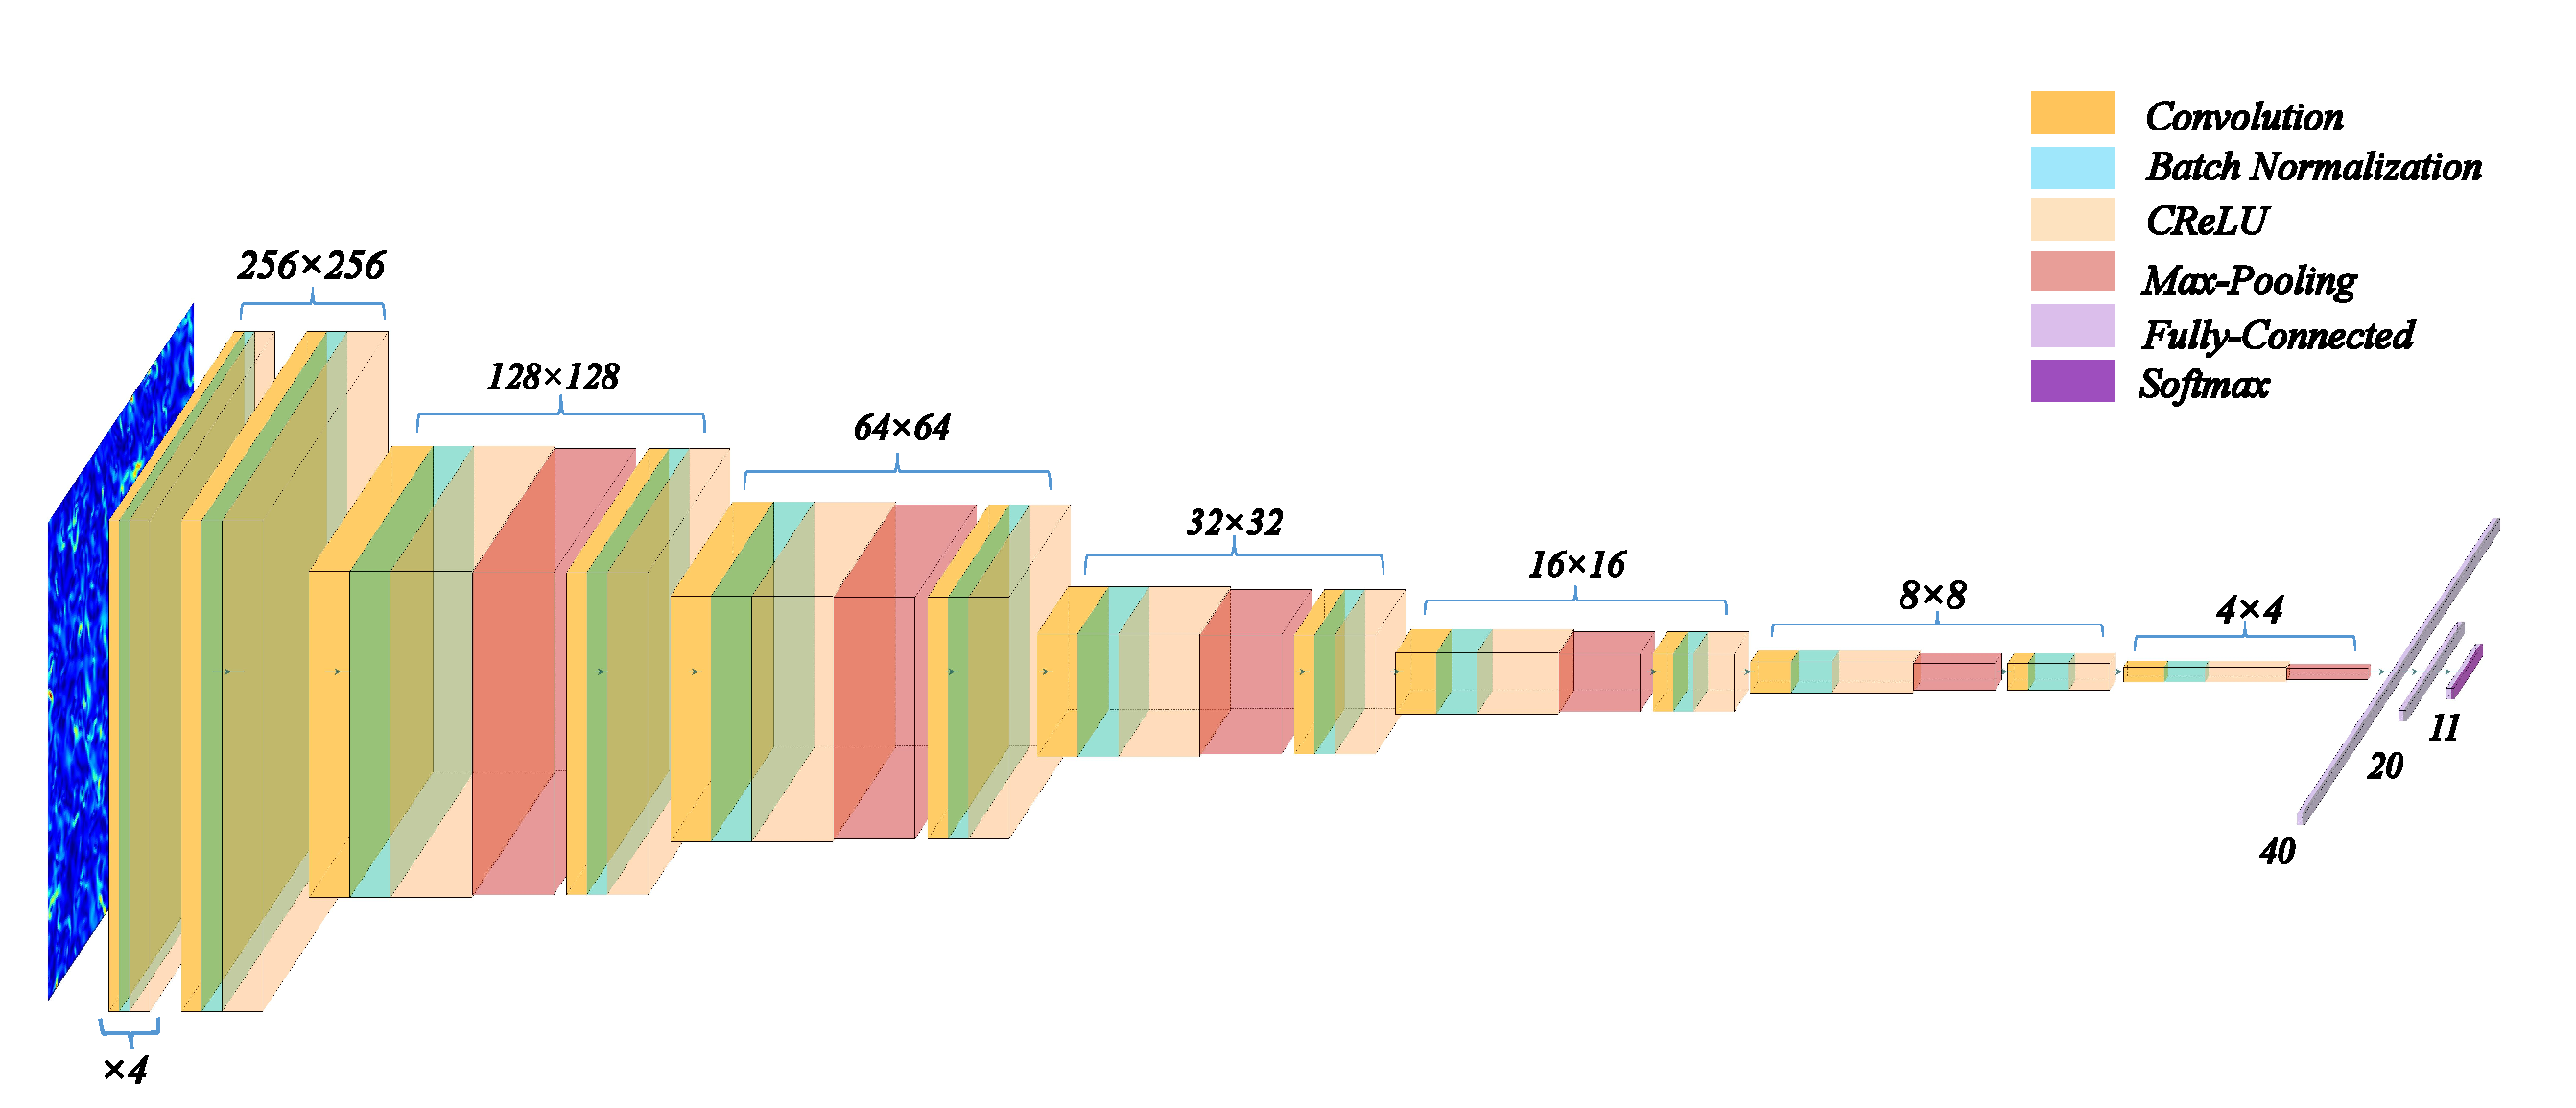
\includegraphics[width=\linewidth , height=0.35\textheight]{figs/arch_vis.pdf}
	\end{center}
	\caption[
			نمایش تجسمی معماری شبکه نهایی و تغییر ابعاد تصویر در طول پیش رفتن در لایه‌های مختلف. طول و عرض حاصل از هر لایه در بالای آن نوشته شده است. عمق هر لایه نیز به ابرپارامترهای آن لایه برمی‌گردد. ورودی شبکه نقشه‌های با ابعاد 
	۲۵۶$\times$۲۵۶
	هستند و خروجی شبکه یا آرایه یک بعدی با ۱۱ عنصر است که هر کدام از عناصر احتمال تعلق داده ورودی به ۱۱ کلاس مختلف از تنش ریسمان را نشان می‌دهد.  
	]{
		نمایش تجسمی معماری شبکه نهایی و تغییر ابعاد تصویر در طول پیش رفتن در لایه‌های مختلف. طول و عرض حاصل از هر لایه در بالای آن نوشته شده است. عمق هر لایه نیز به ابرپارامترهای آن لایه برمی‌گردد. ورودی شبکه نقشه‌های با ابعاد 
		۲۵۶$\times$۲۵۶
		هستند و خروجی شبکه یا آرایه یک بعدی با ۱۱ عنصر است که هر کدام از عناصر احتمال تعلق داده ورودی به ۱۱ کلاس مختلف از تنش ریسمان را نشان می‌دهد.    
		\footnotemark.}
	\label{fig:arch_vis}
\end{figure} 
\footnotetext{برای ساخت این شکل از کد 
	\lr{PlotNeuralNet}
	در لتک استفاده کرده‌ام: \\
	\url{https://github.com/HarisIqbal88/PlotNeuralNet}}
%-------------------------------------------------------------------------
در نتیجه‌ی آزمودن شبکه‌های مختلف به نتایجی دست پیدا کردیم که برای رسیدن به مدل بهینه مفید بودند:
\begin{itemize}
	\item 
	وجود گام یا 
	\lr{stride}
	بزرگتر از ۱ در لایه پیچشی مفیدتر از این است که همه سهم گام‌ها را به لایه ادغام بدهیم. از آن‌جایی که گام بزرگتر از ۱ موجب کاهش بعد تصویر ورودی می‌شود در تعداد گام‌های کل شبکه محدودیت وجود دارد و نمی‌توانیم به همه لایه‌ها سهمی از گام بدهیم.   
	\item
	بهتر است از ادغام بیشینه در شبکه استفاده کنیم. تجربه نشان داده است که ادغام بیشینه بهتر از ادغام میانگین به لبه‌یابی در تصویر کمک می‌کند. 
	\item
	 فیلتر با ابعاد ۵$\times$۵ انتخاب بهینه‌ای است. فیلتر کوچکتر (۳) شبکه را بیش از حد ساده می‌کند و فیلتر بزرگتر (۷) هزینه محاسباتی بسیار بالایی دارد که به استفاده از آن نمی‌ارزد. 
\end{itemize}

پس از طی مراحل طاقت فرسا و زمان‌بر سعی و خطا :) ، به معماری مناسبی برای شبکه عصبی دست یافتیم. 
طبق این دو معیار شبکه‌های مختلف را با هم مقایسه کردیم و در پایان به معماری توصیف شده در جدول 
\ref{Table:arch}
رسیدیم. در شبکه منتخب، در مجموع ۱۶ لایه پیچشی وجود دارد که در ادامه‌ی هر کدام یک لایه ‌BN و لایه تابع فعال‌سازی وجود دارد. علت اینکه تابع فعال‌سازی را به عنوان یک لایه جدا قرار داده‌ایم در حالی که می‌توانست درون لایه پیچشی قرار بگیرد، این است که فعال‌سازی باید بعد از مرحل بهنجارش در BN صورت بگیرد. لایه‌های شبکه در دو بلوک قرار دارند. بلوک اول شامل یک لایه پیچشی( البته به همراه مخلفات!) است که ۴ بار تکرار می‌شود. در این بلوک گام پیچش ۱ است و لایه ادغام نیز وجود ندارد. بنابراین این بلوک منجر به هیچ تغییری در طول و عرض تصویر ورودی نمی‌شود. عمق هر لایه پیچشی  با توجه به تعداد فیلترها مشخص می‌شود و لایه CReLU عمق ورودی را دو برابر می‌کند ولی لایه BN تغییری در عمق ورودی ایجاد نمی‌کند. بلوک دوم شامل ۶ بار تکرار یک الگوست که شامل دو لایه پیچشی است. قسمت اول همانند لایه‌های بلوک اول است اما قسمت دوم شامل لایه پیچشی با گام ۲ است. در انتهای این بلوک یک لایه ادغام با گام ۲ و اندازه ادغام ۲ وجود دارد. لذا بار کاهش ابعاد در این شبکه بر دوش قسمت دوم بلوک دوم است. تصویر پس از گذر از این دو بلوک از لایه‌های پیچشی باید وارد لایه کاملا همبند شود. از ان جایی که خروجی لایه های پیچشی ۲بعدی است و ورودی لایه کاملا همبند باید ۱بعدی است از لایه FLatten  برای تبدیل آرایه دوبعدی به یک بعدی استفاده می‌کنیم. در انتها ۳ لایه کاملا همبند وجود دارد که خروجی لایه آخر یک آرایه یک بعدی با ۱۱ عنصر است، همانگونه که انتظار داشته‌ایم. تابع فعال‌سازی لایه آخر Softmax است که در مسائل طبقه‌بندی چند کلاسه به صورت گسترده به عنوان فعالسازی لایه آخر استفاده می‌شود. شکل
\ref{fig:arch_vis}
چگونگی کاهش ابعاد تصویر ورودی را در طول شبکه نشان می‌دهد.        



%-------------------------------------------------------------------------
\subsection{فرآیند یادگیری}
%----------------------------
\begin{figure}[h!]
	\centering
	\begin{subfigure}{0.5\textwidth}
		\centering
		\includegraphics[scale=0.5]{figs/1_acc_noiseless.png}
		\caption{ تغییرات دقت پیش‌بینی‌ ماشین در طول گام‌های یادگیری.  }
		%		\label{fig:sub1}
	\end{subfigure}%
	\begin{subfigure}{0.5\textwidth}
		\centering
		\includegraphics[scale=0.5]{figs/1_loss_noiseless.jpg}
		\caption{ تغییرات مقدار تابع هزینه در طول گام‌های یادگیری. }
		%		\label{fig:sub2}
	\end{subfigure}
	
	\caption{  تحولات دقت  و مقدار هزینه در طول گام‌های آموزش ماشین 
		برای شبیه‌سازی Healpix ایده‌آل و بدون نوفه. در شکل سمت راست، دقت روی داده‌های آموزش با رنگ سبز و داده‌های آزمون با رنگ قرمز مشخص شده است. مطابق شکل دقت روی داده‌های آزمون گرچه کمی کمتر از  دقت روی داده‌های آموزش است ولی این مقدار تفاوت طبیعی و قابل انتظار است و به معنای برازش بیش از حد نیست. شکل سمت چپ نشان‌دهنده مقادیر تابع هزینه است. مقدار اولیه هزینه، بستگی به انتخاب تابع هزینه دارد. هرچه شدت نوفه بیشتر شود، تابع هزینه به مقادیر بزرگ‌تری همگرا می‌شود.}
	\label{fig:epoch}
\end{figure}
%----------------------------
معماری نهایی مدلی با حدود ۹۰۰۰۰ پارامتر آزاد می‌سازد که آموزش ماشین به معنی پیدا کردن بهترین برازش برای همه این پارامتر‌ها است. این فرآیند برای ورودی‌های با طول و عرض ۲۵۶ پیکسل، به حدودا ۵ ساعت زمان برای اجرا شدن روی یک پردازنده گرافیکی
\LTRfootnote{Graphics processing unit}
\lr{Tesla K80 GPU}
نیاز دارد.
تابع هزینه‌ای که برای آموزش ماشین استفاده کرده‌ایم، تابع Hubber loss معادله
\ref{huber_loss}
است. گرچه نتایج تابع هزینه Cross Entropy معادله
\ref{CE_loss}
 و Logloss 
%\ref{CE_loss}
 نیز امیدبخش بوده است. از AdamOptimizer نیز برای بهینه‌سازی استفاده شده است. مقدار نرخ یادگیری را در ابتدای فرآیند آموزش $0.001$ قرار دادیم و در حین یادگیری هر زمانی که مقدار هزینه در چند مرحله از یادگیری ثابت ماند و پیشرفت زیادی نکرد به مرور کاهش دادیم. نرخ یادگیری تا مقدار $0.000005$ نیز کاهش پیدا می‌کند.
 در طول فرآیند آموزش همواره باید خطر برازش بیش از حد را مدّ نظر قرار داد. برای اینکه مطمئن باشیم برازش بیش از اندازه رخ نداده است باید همواره در بازه‌های زمانی کوتاه دقت روی داده‌های آموزش و روی داده‌های آزمون را مقایسه کنیم. اگر تفاوت معنی‌دار (به طور مثال حداکثر بیش از ۱۰ درصد تفاوت) وجود داشت به این معنی است که مدل در حال برازش بیش از حد شدن است. ترسیم ماتریس درهم‌ریختگی برای داده‌های آموزش و آزمون هم راه دقیقی برای سنجش برازش ماشین است. در مدلی که به برازش بیش از حد دچار نباشد نباید تفاوت فاحشی بین این دو ماتریس وجود داشته باشد. 
  در شکل 
\ref{fig:epoch} 
تحول مقدار هزینه در طول زمان یادگیری و هم‌چنین تغییرات دقت ماشین برای داده‌های Healpix بدون نوفه و کاملا ایده‌آل نشان داده ‌شده است. فرآیند ساخت مدل و آموزش آن توسط بسته نرم‌افزاری تنسورفلو
\LTRfootnote{Tensorflow :\url{www.tensorflow.org}}
\cite{abadi2016tensorflow}
و در محیط پایتون انجام شده است. برای سهولت بیشتر در کار با تنسورفلو، از بسته نرم‌افزاری 
Ngene 
\LTRfootnote{\url{github.com/vafaei-ar/Ngene.git}}
استفاده شده است. کدهای مربوط به این تحقیق در گیت‌هاب
\LTRfootnote{github}
 به آدرس
\url{github.com/M-Torki/DeePlanck.git }
در دسترس است.
  
  
  
  \section{نتایج آموزش ماشین روی داده‌های شبیه‌سازی }
  \label{sec:results}
  
  مطابق روشی که در این فصل شرح داده شد و پس از آن که به یک معماری بهینه برای شبکه پیچشی رسیدیم، شبکه را برای انواع شبیه‌سازی‌هایی که در این تحقیق مدّ نظر است به صورت جداگانه آموزش دادیم. پس از اجرای فرآیند آموزش، متناظر با هر دسته شبیه‌سازی به یک مدل نهایی دست پیدا کردیم. برای گزارش دقت هر مدل و حدی از تنش ریسمان که ماشین قادر به دیدن و تشخیص آن است از دو معیار مقدار پی و ماتریس درهم‌ریختگی استفاده کرده‌ایم که متناظر با هر کدام از این معیارها ۲ کمیت معرفی می‌کنیم:
  \begin{description}
  	\item
  	کمینه قابل اندازه‌گیری یا $G\mu_{mes}$:\\
  	این کمیت برای ماتریس درهم‌ریختگی تنشی است که ماشین با $\%$۹۵ دقت ($\sigma$2) توانایی تشخیص و اندازه‌گیری آن را دارد. این مقدار در ماتریس معادل کلاسی است که آرایه روی قطر متناظر با آن $\%$۹۵ باشد. از آن‌جایی که مقادیر روی قطر گاهی کمی کمتر یا بیشتر از $\%$۹۵ هستند برای به دست آوردن حدود تنشی که دقت اندازه‌گیری آن دقیقا مساوی ۹۵ شود مقادیر روی قطر ماتریس را درون‌یابی می‌کنیم. در اینجا ما برای ساده‌سازی فرض می‌کنیم که رفتار تابع خطی است.
  	علاوه بر ماتریس درهم‌ریختگی، حد کمینه قابل اندازه‌گیری را می‌توان با اطلاعات مقادیر پی برای کلاس‌های مختلف به دست آورد. طبق تعریف ما مقدار تنشی که قابل اندازه گیری است لزوما باید از تمام کلاس‌های دیگر قابل تمایز باشد. یعنی مقدار پی بین توزیع مربوط به این مقدار کمینه و توزیع تمام کلاس‌های دیگر کمتر از $0.05$ باشد که معادل دقت $\sigma$2 است. همانند روش به دست آوردین کمینه قابل اندازه‌گیری با ماتریس، برای محاسبه مقدار دقیق این حد با مقدار پی باید درون‌یابی انجام دهیم.     
  	\item
  	کمینه قابل آشکارسازی یا $G\mu_{det}$:\\
  	آشکارسازی به معنای تشخیص دادن نقشه‌های ریسمان‌دار از نقشه‌ی پوچ و بدون ریسمان است. مشابه حد قابل اندازه‌گیری، این حد را هم از دو منظر ماتریس درهم‌ریختگی و مقدار پی به دست می‌آوریم. از منظر ماتریس درهم‌ریختگی، حد قابل آشکارسازی مقدار تنشی است که کمتر از $\%$۵ نمونه‌های مربوط به آن با کلاس پوچ یا صفر توسط ماشین اشتباه گرفته شده باشد. به عبارتی مقادیر ستون اول در ماتریس برای ما مهم است. اولین کلاسی که آرایه مربوط به آن در ستون اول کوچکتر یا مساوی $0.05$ باشد حد قابل آشکارسازی را مشخص می‌کند. برخلاف قبل که گفتیم مقادیر را درون‌یابی کرده‌ایم، برای این حد به گزارش برچسب کلاس مربوطه اکتفا می‌کنیم. حد قابل آشکارسازی توسط مقادیر پی نیز قابل محاسبه است. برای این کار توزیع پیش‌بینی‌های مربوط به هر کلاس را با توزیع پیش‌بینی‌های کلاس صفر یا پوچ مقایسه می کنیم و مقدار پی مربوطه را به دست می‌آوریم. آستانه مورد نظر در این مورد هم دقت $\sigma$2 یا همان مقدار پی $0.05$ است.   	    
  \end{description}
  در بخش بعدی حدود قابل اندازه‌گیری و حدود قابل آشکارسازی را برای ۷ حالت شبیه‌سازی مختلفی که بررسی کرده‌ایم بیان خواهیم کرد. ماتریس در‌هم‌ریختگی و نمودار‌های مربوط به مقدار پی نیز برای همه شبیه‌سازی‌ها آورده شده است.  
%  \newpage  
  %-------------------------------------------------------------------------
  \subsection{حدود قابل اندازه‌گیری و قابل آشکارسازی به دست آمده}
  \label{subsec:upper_bounds}
  
\subsubsection{آزمایش شبه نسل چهارم تابش زمینه-نوع دوم}
نتایج به دست آمده برای آزمایش شبه نوع دوم نسل چهار، با\\
$N_{side} = 4096$ \\
$SNR=20$\\
$FWHM = 0.9'$
به شرح زیر است:\\
قدرت اندازه‌گیری مدل با معیار ماتریس در‌هم‌ریختگی مقدار 
$G\mu \geq 1.9\times 10^{-7}$
و با معیار مقدار پی 
$G\mu \geq 1.7\times 10^{-7}$
است. هم‌چنین قدرت آشکارسازی مدل با معیار ماتریس در‌هم‌ریختگی مقدار
$G\mu \geq 8.9\times 10^{-8}$
و با معیار مقدار پی 
$G\mu \geq 2.6\times 10^{-8}$
است. اطلاعات مربوط به مقادیر پی در شکل
\ref{fig:s4ii_pv}
و اطلاعات ماتریس درهم‌ریختگی در شکل
\ref{fig:s4ii_cm}
 آمده است.
  	
  	\begin{figure}
  		\centering
  		\begin{subfigure}{0.5\textwidth}
  			\centering
  			\includegraphics[scale=0.5]{figs/pv_m_s4ii.png}
  			\caption{   کمینه تنش قابل اندازه‌گیری برای آزمایش
  				\\	 شبه نوع دوم نسل چهار
  				بر اساس آمار \lr{P\;value}}
  			%		\label{fig:sub1}
  		\end{subfigure}%
  		\begin{subfigure}{0.5\textwidth}
  			\centering
  			\includegraphics[scale=0.5]{figs/pv_d_s4ii.png}
  			\caption{  کمینه تنش قابل آشکارسازی برای آزمایش 
  				\\ شبه نوع دوم نسل چهار
  				بر اساس آمار \lr{P\;value} }
  			%		\label{fig:sub2}
  		\end{subfigure}
  		
  		\caption{حدود قابل اندازه‌گیری و آشکارسازی برای آزمایش شبه نوع دوم نسل چهارم تابش زمینه
  			به وسیله درون‌یابی مقادیر پی.}
  		\label{fig:s4ii_pv}
  	\end{figure}
  	%------------------------
  	\begin{figure}
  		\centering
  		\begin{subfigure}{\textwidth}
  			\centering
  			\includegraphics[scale=0.7]{figs/cm_s4ii.png}
  			\caption{  ماتریس درهم‌ریختگی برای  
  			آزمایش شبه نوع دوم نسل چهار}
  			%		\label{fig:sub1}
  		\end{subfigure}%
  		
  		\begin{subfigure}{0.5\linewidth}
  			\centering
  			\includegraphics[width=\textwidth , height=0.22\textheight]{figs/cm_m_s4ii.png}
  			\caption{  کمینه تنش قابل اندازه‌گیری توسط ماشین برای آزمایش شبه نوع دوم نسل چهار}
  			%		\label{fig:sub2}
  		\end{subfigure}
  		
  		\caption{ماتریس در هم ریختگی برای دسته‌بندی داده‌های آزمایش شبه نوع دوم نسل چهارم تابش زمینه
  			و به دست آوردن حد کمینه قابل اندازه‌گیری توسط ماشین از روی این ماتریس به وسیله درون‌یابی عناصر قطر.}
  		\label{fig:s4ii_cm}
  	\end{figure}
  	
  	
  	
  	%-------------------------------------------------------------------------
  	\subsubsection{آزمایش شبه نسل چهارم تابش زمینه-نوع اول} 
  	نتایج به دست آمده برای آزمایش شبه نوع اول نسل چهار، با\\
  	$N_{side} = 4096$ \\
  	$SNR=15$\\
   	$FWHM = 0.9'$
  	به شرح زیر است:\\
  	قدرت اندازه‌گیری مدل با معیار ماتریس در‌هم‌ریختگی مقدار 
  	$G\mu \geq 1.9\times 10^{-7}$
  	و با معیار مقدار پی 
  	$G\mu \geq 1.6\times 10^{-7}$
  	است. هم‌چنین قدرت آشکارسازی مدل با معیار ماتریس در‌هم‌ریختگی مقدار
  	$G\mu \geq 1.9\times 10^{-7}$
  	و با معیار مقدار پی 
  	$G\mu \geq 1.3\times 10^{-7}$
  	است. اطلاعات مربوط به مقادیر پی در شکل
  	\ref{fig:s4i_pv}
  	و اطلاعات ماتریس درهم‌ریختگی در شکل
  	\ref{fig:s4i_cm}
  	آمده است.
  	
  	
  	
  	\begin{figure}
  		\centering
  		\begin{subfigure}{0.5\textwidth}
  			\centering
  			\includegraphics[scale=0.5]{figs/pv_m_s4i.png}
  			\caption{   کمینه تنش قابل اندازه‌گیری برای آزمایش 
  				\\	 شبه نوع اول نسل چهار
  				بر اساس آمار \lr{P\;value}}
  			%		\label{fig:sub1}
  		\end{subfigure}%
  		\begin{subfigure}{0.5\textwidth}
  			\centering
  			\includegraphics[scale=0.5]{figs/pv_d_s4i.png}
  			\caption{  کمینه تنش قابل آشکارسازی برای آزمایش 
  				\\  شبه نوع اول نسل چهار
  				بر اساس آمار \lr{P\;value} }
  			%		\label{fig:sub2}
  		\end{subfigure}
  		
  		\caption{حدود قابل اندازه‌گیری و آشکارسازی برای آزمایش 
شبه نوع اول نسل چهارم تابش زمینه به وسیله درون‌یابی مقادیر پی.}
  		\label{fig:s4i_pv}
  	\end{figure}
  	%------------------------
  	\begin{figure}
  		\centering
  		\begin{subfigure}{\textwidth}
  			\centering
  			\includegraphics[scale=0.7]{figs/cm_s4i.png}
  			\caption{  ماتریس درهم‌ریختگی برای آزمایش 
  				شبه نوع اول نسل چهار }
  			%		\label{fig:sub1}
  		\end{subfigure}%
  		
  		\begin{subfigure}{0.5\linewidth}
  			\centering
  			\includegraphics[width=\textwidth , height=0.22\textheight]{figs/cm_m_s4i.png}
  			\caption{  کمینه تنش قابل اندازه‌گیری توسط ماشین برای آزمایش 
  				شبه نوع اول نسل چهار }
  			%		\label{fig:sub2}
  		\end{subfigure}
  		
  		\caption{ماتریس در هم ریختگی برای دسته‌بندی داده‌های آزمایش
شبه نوع اول نسل چهارم تابش زمینه و به دست آوردن حد کمینه قابل اندازه‌گیری توسط ماشین از روی این ماتریس به وسیله درون‌یابی عناصر قطر.}
  		\label{fig:s4i_cm}
  	\end{figure}
  	
  	
  	
  	
  	%-------------------------------------------------------------------------
  	
\subsubsection{آزمایش‌ شبه تلسکوپ کیهان‌شناسی آتاکاما}
  	نتایج به دست آمده برای آزمایش شبه تلسکوپ کیهان‌شناسی آتاکاما ، با\\
  	$N_{side} = 4096$ \\
  	$SNR=10$\\
  	$FWHM = 0.9'$
  	به شرح زیر است:\\
  	قدرت اندازه‌گیری مدل با معیار ماتریس در‌هم‌ریختگی مقدار 
  	$G\mu \geq 4.1\times 10^{-7}$
  	و با معیار مقدار پی 
  	$G\mu \geq 3.5\times 10^{-7}$
  	است. هم‌چنین قدرت آشکارسازی مدل با معیار ماتریس در‌هم‌ریختگی مقدار
  	$G\mu \geq 1.9\times 10^{-7}$
  	و با معیار مقدار پی 
  	$G\mu \geq 2.4\times 10^{-7}$
  	است.
  	اطلاعات مربوط به مقادیر پی در شکل
  	\ref{fig:act_pv}
  	و اطلاعات ماتریس درهم‌ریختگی در شکل
  	\ref{fig:act_cm}
  	آمده است.
  	
  	\begin{figure}
  		\centering
  		\begin{subfigure}{0.5\textwidth}
  			\centering
  			\includegraphics[scale=0.5]{figs/pv_m_act.png}
  			\caption{   کمینه تنش قابل اندازه‌گیری برای آزمایش  
  				\\	شبه تلسکوپ آتاکاما
  				بر اساس آمار \lr{P\;value} }
  			%		\label{fig:sub1}
  		\end{subfigure}%
  		\begin{subfigure}{0.5\textwidth}
  			\centering
  			\includegraphics[scale=0.5]{figs/pv_d_act.png}
  			\caption{  کمینه تنش قابل آشکارسازی برای آزمایش 
  				\\ شبه تلسکوپ آتاکاما
  				بر اساس آمار 
  				\lr{P\;value}. }
  			%		\label{fig:sub2}
  		\end{subfigure}
  		
  		\caption{حدود قابل اندازه‌گیری و آشکارسازی برای آزمایش 
شبه تلسکوپ آتاکاما به وسیله درون‌یابی مقادیر پی.}
  		\label{fig:act_pv}
  	\end{figure}
  	%------------------------
  	\begin{figure}
  		\centering
  		\begin{subfigure}{\textwidth}
  			\centering
  			\includegraphics[scale=0.7]{figs/cm_act.png}
  			\caption{  ماتریس درهم‌ریختگی برای آزمایش شبه تلسکوپ آتاکاما }
  			%		\label{fig:sub1}
  		\end{subfigure}%
  		
  		\begin{subfigure}{0.5\linewidth}
  			\centering
  			\includegraphics[width=\textwidth , height=0.22\textheight]{figs/cm_m_act.png}
  			\caption{  کمینه تنش قابل اندازه‌گیری توسط ماشین برای آزمایش شبه تلسکوپ آتاکاما }
  			%		\label{fig:sub2}
  		\end{subfigure}
  		
  		\caption{ماتریس در هم ریختگی برای دسته‌بندی داده‌های آزمایش شبه تلسکوپ آتاکاما
  			و به دست آوردن حد کمینه قابل اندازه‌گیری توسط ماشین از روی این ماتریس به وسیله درون‌یابی عناصر قطر.}
  		\label{fig:act_cm}
  	\end{figure}
  	
  	
  	%-------------------------------------------------------------------------
  	
  \subsubsection{  	شبیه‌سازی  \lr{FFP10}}
   	\begin{itemize}
   		\item \textbf{حالت ایده‌آل بدون نوفه} \\
   		   	نتایج به دست آمده برای شبیه‌سازی‌های بدون نوفه
   		   	\lr{FFP10}
   		   	با\\
   		$N_{side} = 2048$ \\
   		$FWHM = 5'$
   		  به شرح زیر است:\\
   		قدرت اندازه‌گیری مدل با معیار ماتریس در‌هم‌ریختگی مقدار 
   		$G\mu \geq 8.6\times 10^{-8}$
   		و با معیار مقدار پی 
   		$G\mu \geq 8.1\times 10^{-8}$
   		است. هم‌چنین قدرت آشکارسازی مدل با معیار ماتریس در‌هم‌ریختگی مقدار
   		$G\mu \geq 4.1\times 10^{-8}$
   		و با معیار مقدار پی 
   		$G\mu \geq 3.2\times 10^{-8}$
   		است.
   		اطلاعات مربوط به مقادیر پی در شکل
   		\ref{fig:ffp_pv}
   		و اطلاعات ماتریس درهم‌ریختگی در شکل
   		\ref{fig:ffp_cm}
   		آمده است.
   		
		\item \textbf{با نوفه رصدی} \\
		نتایج به دست آمده برای شبیه‌سازی‌های \lr{FFP10}
		با\\
		 $N_{side} = 2048$ \\
 		 $SNR=10$\\
		 $FWHM = 5'$\\
		 به شرح زیر است:\\
		 قدرت اندازه‌گیری مدل با معیار ماتریس در‌هم‌ریختگی مقدار 
		 $G\mu \geq 6.8\times 10^{-7}$
		 و با معیار مقدار پی 
		 $G\mu \geq 3.6\times 10^{-7}$
		 است. هم‌چنین قدرت آشکارسازی مدل با معیار ماتریس در‌هم‌ریختگی مقدار
		 $G\mu \geq 4.1\times 10^{-7}$
		 و با معیار مقدار پی 
		 $G\mu \geq 1.4\times 10^{-7}$
		 است.
		 اطلاعات مربوط به مقادیر پی در شکل
		 \ref{fig:nffp_pv}
		 و اطلاعات ماتریس درهم‌ریختگی در شکل
		 \ref{fig:nffp_cm}
		 آمده است.
		
		 
   	\end{itemize}

  	
  	\begin{figure}
  		\centering
  		\begin{subfigure}{0.5\textwidth}
  			\centering
  			\includegraphics[scale=0.5]{figs/pv_m_ffp.png}
  			\caption{   کمینه تنش قابل اندازه‌گیری برای شبیه‌سازی 
  				\\	\lr{FFP10} 
  				بدون نوفه بر اساس آمار 
  				\lr{P\;value}. }
  			%		\label{fig:sub1}
  		\end{subfigure}%
  		\begin{subfigure}{0.5\textwidth}
  			\centering
  			\includegraphics[scale=0.5]{figs/pv_d_ffp.png}
  			\caption{  کمینه تنش قابل آشکارسازی برای شبیه‌سازی 
  				\\	\lr{FFP10} 
  				بدون نوفه بر اساس آمار 
  				\lr{P\;value}. }
  			%		\label{fig:sub2}
  		\end{subfigure}
  		
  		\caption{حدود قابل اندازه‌گیری و آشکارسازی برای شبیه‌سازی 
  					\lr{FFP10} 
  			بدون نوفه به وسیله درون‌یابی مقادیر پی}
  		\label{fig:ffp_pv}
  	\end{figure}
  	%------------------------
  	\begin{figure}
  		\centering
  		\begin{subfigure}{0.5\textwidth}
  			\centering
  			\includegraphics[scale=0.5]{figs/pv_m_nffp.png}
  			\caption{   کمینه تنش قابل اندازه‌گیری برای شبیه‌سازی 
  				\\	\lr{FFP10} 
  				بر اساس آمار 
  				\lr{P\;value} }
  			%		\label{fig:sub1}
  		\end{subfigure}%
  		\begin{subfigure}{0.5\textwidth}
  			\centering
  			\includegraphics[scale=0.5]{figs/pv_d_nffp.png}
  			\caption{  کمینه تنش قابل آشکارسازی برای شبیه‌سازی 
  				\\	\lr{FFP10} 
  				بر اساس آمار 
  				\lr{P\;value} }
  			%		\label{fig:sub2}
  		\end{subfigure}
  		
  		\caption{حدود قابل اندازه‌گیری و آشکارسازی برای شبیه‌سازی 
  				\lr{FFP10} 
  			به وسیله درون‌یابی مقادیر پی.}
  		\label{fig:nffp_pv}
  	\end{figure}
  	%------------------------
  	\begin{figure}
  		\centering
  		\begin{subfigure}{\textwidth}
  			\centering
  			\includegraphics[scale=0.7]{figs/cm_ffp.png}
  			\caption{  ماتریس درهم‌ریختگی برای شبیه‌سازی 
  					\lr{FFP10} 
  				بدون نوفه }
  			%		\label{fig:sub1}
  		\end{subfigure}%
  		
  		\begin{subfigure}{0.5\linewidth}
  			\centering
  			\includegraphics[width=\textwidth , height=0.22\textheight]{figs/cm_m_ffp.png}
  			\caption{  کمینه تنش قابل اندازه‌گیری توسط ماشین برای شبیه‌سازی 
  					\lr{FFP10} 
  				بدون نوفه }
  			%		\label{fig:sub2}
  		\end{subfigure}
  		
  		\caption{ماتریس در هم ریختگی برای دسته‌بندی داده‌های شبیه‌سازی
  			  		\lr{FFP10}  
  			بدون نوفه و به دست آوردن حد کمینه قابل اندازه‌گیری توسط ماشین از روی این ماتریس به وسیله درون‌یابی عناصر قطر.}
  		\label{fig:ffp_cm}
  	\end{figure}
  	%------------------------
  	\begin{figure}
  		\centering
  		\begin{subfigure}{\textwidth}
  			\centering
  			\includegraphics[scale=0.7]{figs/cm_nffp.png}
  			\caption{  ماتریس درهم‌ریختگی برای شبیه‌سازی 
  				  	\lr{FFP10}  
  			}
  			%		\label{fig:sub1}
  		\end{subfigure}%
  		
  		\begin{subfigure}{0.5\linewidth}
  			\centering
  			\includegraphics[width=\textwidth , height=0.22\textheight]{figs/cm_m_nffp.png}
  			\caption{  کمینه تنش قابل اندازه‌گیری توسط ماشین برای شبیه‌سازی 
  					\lr{FFP10} 
  			}
  			%		\label{fig:sub2}
  		\end{subfigure}
  		
  		\caption{ماتریس در هم ریختگی برای دسته‌بندی داده‌های شبیه‌سازی
  					\lr{FFP10} 
  			و به دست آوردن حد کمینه قابل اندازه‌گیری توسط ماشین از روی این ماتریس به وسیله درون‌یابی عناصر قطر.}
  		\label{fig:nffp_cm}
  	\end{figure}
  	
  	%-------------------------------------------------------------------------
  	
    	
  \subsubsection{  	شبیه‌سازی End-to-End }
  \begin{itemize}
  	\item \textbf{حالت ایده‌آل بدون نوفه} \\
  	نتایج به دست آمده برای شبیه‌سازی‌های بدون نوفه
  	\lr{E2E}
  	با\\
  	$N_{side} = 2048$ \\
  	$FWHM = 5'$
  	به شرح زیر است:\\
  	قدرت اندازه‌گیری مدل با معیار ماتریس در‌هم‌ریختگی مقدار 
  	$G\mu \geq 7.2\times 10^{-7}$
  	و با معیار مقدار پی 
  	$G\mu \geq 1.9\times 10^{-7}$
  	است. هم‌چنین قدرت آشکارسازی مدل با معیار ماتریس در‌هم‌ریختگی مقدار
  	$G\mu \geq 4.1\times 10^{-7}$
  	و با معیار مقدار پی 
  	$G\mu \geq 1.4\times 10^{-7}$
  	است.
  	اطلاعات مربوط به مقادیر پی در شکل
  	\ref{fig:e2eless_pv}
  	و اطلاعات ماتریس درهم‌ریختگی در شکل
  	\ref{fig:E2Eless_cm}
  	آمده است.
  	
  	\item \textbf{با نوفه رصدی} \\
  	نتایج به دست آمده برای شبیه‌سازی‌های \lr{E2E}
  	با\\
  	$N_{side} = 2048$ \\
  	$SNR=8$\\
  	$FWHM = 5'$\\
  	به شرح زیر است:\\
  	قدرت اندازه‌گیری مدل با معیار ماتریس در‌هم‌ریختگی مقدار 
  	$G\mu \geq 8.8\times 10^{-7}$
  	و با معیار مقدار پی 
  	$G\mu \geq 4.9\times 10^{-7}$
  	است. هم‌چنین قدرت آشکارسازی مدل با معیار ماتریس در‌هم‌ریختگی مقدار
  	$G\mu \geq 8.8\times 10^{-7}$
  	و با معیار مقدار پی 
  	$G\mu \geq 3.7\times 10^{-7}$
  	است.
  	اطلاعات مربوط به مقادیر پی در شکل
  	\ref{fig:nsyE2E_pv}
  	و اطلاعات ماتریس درهم‌ریختگی در شکل
  	\ref{fig:nsye2e_cm}
  	آمده است.
  	
  	
  \end{itemize}
  	
  	\begin{figure}
  		\centering
  		\begin{subfigure}{0.5\textwidth}
  			\centering
  			\includegraphics[scale=0.5]{figs/pv_m_e2eless.png}
  			\caption{   کمینه تنش قابل اندازه‌گیری برای شبیه‌سازی 
  				\\			\lr{E2E}
  				بدون نوفه بر اساس آمار
  				\lr{P\;value} }
  			%		\label{fig:sub1}
  		\end{subfigure}%
  		\begin{subfigure}{0.5\textwidth}
  			\centering
  			\includegraphics[scale=0.5]{figs/pv_d_e2eless.png}
  			\caption{  کمینه تنش قابل آشکارسازی برای شبیه‌سازی 
  				\\ 		\lr{E2E}
  				بدون نوفه بر اساس آمار
  				\lr{P\;value}	
  			}
  			%		\label{fig:sub2}
  		\end{subfigure}
  		
  		\caption{حدود قابل اندازه‌گیری و آشکارسازی برای شبیه‌سازی 
  			\lr{E2E}
  			بدون نوفه به وسیله درون‌یابی مقادیر پی.}
  		\label{fig:e2eless_pv}
  	\end{figure}
  	%------------------------
  	\begin{figure}[H]
  		\centering
  		\begin{subfigure}{0.5\textwidth}
  			\centering
  			\includegraphics[scale=0.5]{figs/pv_m_nsye2e.png}
  			\caption{   کمینه تنش قابل اندازه‌گیری برای شبیه‌سازی 
  				\\			\lr{E2E}
  				بر اساس آمار
  				\lr{P\;value} }
  			%		\label{fig:sub1}
  		\end{subfigure}%
  		\begin{subfigure}{0.5\textwidth}
  			\centering
  			\includegraphics[scale=0.5]{figs/pv_d_nsye2e.png}
  			\caption{  کمینه تنش قابل آشکارسازی برای شبیه‌سازی 
  				\\ 		\lr{E2E}
  				بر اساس آمار 
  				\lr{P\;value}	
  			}
  			%		\label{fig:sub2}
  		\end{subfigure}
  		
  		\caption{حدود قابل اندازه‌گیری و آشکارسازی برای شبیه‌سازی 
				\lr{E2E}
  			به وسیله درون‌یابی مقادیر پی .}
  		\label{fig:nsyE2E_pv}
  	\end{figure}
  	%------------------------
  	\begin{figure}[H]
  		\centering
  		\begin{subfigure}{\textwidth}
  			\centering
  			\includegraphics[scale=0.7]{figs/cm_e2eless.png}
  			\caption{  ماتریس درهم‌ریختگی برای شبیه‌سازی 
					\lr{E2E}
  				بدون نوفه }
  			%		\label{fig:sub1}
  		\end{subfigure}%
  		
  		\begin{subfigure}{0.5\linewidth}
  			\centering
  			\includegraphics[width=\textwidth , height=0.22\textheight]{figs/cm_m_e2eless.png}
  			\caption{  کمینه تنش قابل اندازه‌گیری توسط ماشین برای شبیه‌سازی 
					\lr{E2E}	
  				بدون نوفه }
  			%		\label{fig:sub2}
  		\end{subfigure}
  		
  		\caption{ماتریس در هم ریختگی برای دسته‌بندی داده‌های شبیه‌سازی
\lr{E2E}
  			بدون نوفه 
  			و به دست آوردن حد کمینه قابل اندازه‌گیری توسط ماشین از روی این ماتریس به وسیله درون‌یابی عناصر قطر.}
  		\label{fig:e2eless_cm}
  	\end{figure}
  	%------------------------
  	\begin{figure}[H]
  		\centering
  		\begin{subfigure}{\textwidth}
  			\centering
  			\includegraphics[scale=0.7]{figs/cm_nsye2e.png}
  			\caption{  ماتریس درهم‌ریختگی برای شبیه‌سازی 
					\lr{E2E}
  			}
  			%		\label{fig:sub1}
  		\end{subfigure}%
  		
  		\begin{subfigure}{0.5\linewidth}
  			\centering
  			\includegraphics[width=\textwidth , height=0.22\textheight]{figs/cm_m_nsye2e.png}
  			\caption{  کمینه تنش قابل اندازه‌گیری توسط ماشین برای شبیه‌سازی 
					\lr{E2E}
  			}
  			%		\label{fig:sub2}
  		\end{subfigure}
  		
  		\caption{ماتریس در هم ریختگی برای دسته‌بندی داده‌های شبیه‌سازی
\lr{E2E}
  			و به دست آوردن حد کمینه قابل اندازه‌گیری توسط ماشین از روی این ماتریس به وسیله درون‌یابی عناصر قطر.
  		}
  		\label{fig:nsye2e_cm}
  	\end{figure}
  	
  	%------------------------
  	
  	
  	%-------------------------------------------------------------------------


\section{اعمال مدل روی داده‌های پلانک ۲۰۱۸}
\label{sec:data_results}
استراتژی ما در این تحقیق این است که با استفاده از مدلی که به وسیله نقشه‌های شبیه‌سازی ساخته شده‌ است، مقدار تنش ریسمان موجود در داده‌های رصدی را اندازه‌گیری کنیم و یا حد بالایی برای آن بگذاریم. تا این مرحله ما توانسته‌ایم متناظر با هر یک از شبیه‌سازی‌های نسل چهارم تابش زمینه، تلسکوپ آتاکاما و همینطور شبیه‌سازی‌های پلانک مدل‌‌سازی انجام دهیم. حال باید این مدل‌ها را بر روی داده‌های رصدی اعمال کنیم. از آن‌جایی که داده‌های رصدی تابش زمینه پلانک ۲۰۱۸
\cite{calabrese2019planck}
جدیدترین و دقیق‌ترین داده‌ها در این زمان است، ما از نقشه‌های رصدی ماهواره پلانک استفاده می‌کنیم. ۴ دسته از داده‌های رصدی موجود است که در روش تفکیک مولفه با هم تفاوت دارند. این ۴ روش عبارتند از 
SMICA, NILC , SEVEM 
و 
Commander.
از آن‌جایی که این ۴ دسته از نقشه‌های رصدی برتری مشخصی نسبت به یکدیگر ندارند ما برای این تحقیق نقشه‌های تفکیک مولفه
\lr{SMICA}
\LTRfootnote{pla.esac.esa.int $\to$ maps $\to$ CMB maps $\to$ SMICA}
را انتخاب کرده‌ایم که وضوح آن ۵ دقیقه قوسی است.
بخشی از آسمانِ تابش زمینه توسط صفحه کهکشان و یا تعدادی از اجرام بسیار پرنور پوشانده شده و اطلاعات مربوط به دمای این محدوده و نقاط از دست رفته است. در حین کار کردن با داده‌های رصدی توجه به این مسئله حائز اهمیت است. قبل از آن که داده‌ها را به ماشین بدهیم تا پیش‌بینی آن را دریافت کنیم، لازم است که تکه‌هایی از آسمان که بیش از حد مشخصی پوشانده شده اند را از داده‌ها به کلی حذف کنیم. برای این کار نقشه‌ای از نقاط پوشانده شده آسمان در گنجینه پلانک تحت عنوان \gu{نقشه ماسک}
\LTRfootnote{pla.esac.esa.int $\to$ maps $\to$ mask $\to$ cmb $\to$ 2018\;component\;separation\;common\;mask\;in\;intensity}
 موجود است. ماسک نقشه‌ای است که مقدار آن در تمامی پیکسل‌ها ۱ است، جز پیکسل‌هایی که پوشانده شده اند. که این پیکسل‌های پوشیده شده مقدار صفر دارند. ما برای اینکه داده‌ی رصدی را به ماشین بدهیم لازم داریم که تمام فرآیندهایی که روی ورودی‌های ماشین (که شبیه‌سازی‌ها بودند) انجام داده‌ایم را روی داده رصدی نیز تکرار کنیم. پس در ابتدا باید نقشه آسمان را که
  $ N_{side} = 2048$ 
  	را به تکه‌های
 	 256$\times$256
 	  تقسیم کنیم. برای اعمال کردن اثر ماسک، باید تکه‌هایی که شدت ماسک شدن آن‌ها زیاد است را حذف کنیم. آستانه‌ای که ما برای ماسک کردن قرارداد کرده‌ایم، مقدار $\%$ ۹۵ است. به عبارتی تکه‌هایی از آسمان که بیش از $\%$۹۵ پیکسل‌های آن‌ها   پوشانده شده باشد را حذف می‌کنیم. در این تکه‌ها از آسمان میانگین مقادیر پیکسل‌ها کمتر از $0.95$ است. در این فرآیند تقریبا $\%$۶۴ آسمان که معادل ۴۸۹ تکه  256$\times$256 است باقی می‌ماند.
 	  \\
 	  گفتیم که تمام پیش‌پردازش‌هایی که بر روی داده‌های شبیه‌سازی انجام شده است باید عیناً برای داده‌های رصدی نیز تکرار شود. لذا پس از تکه تکه کردن آسمان با ابعاد ۲۵۶ و اعمال اثر ماسک، باید این تکه‌ها را با فیلتر شار پردازش کنیم. در آخر نیز لازم است تصاویر فیلتر شده را همانند داده‌های آموزش بهنجار کنیم. 
 	  		%------------------------
 	
 \begin{figure}
 	\centering
 	\begin{subfigure}{0.5\textwidth}
 		\centering
 		\includegraphics[scale=0.25]{figs/smica.png}
 		\caption{آسمانِ تابش زمینه رصدی}
 		%		\label{fig:sub1}
 	\end{subfigure}%
 	\begin{subfigure}{0.5\textwidth}
 		\centering
 		\includegraphics[scale=0.25]{figs/mask.png}
 		\caption{ نقشه ماسک }
 		%		\label{fig:sub2}
 	\end{subfigure}
 	
 	\caption{ داده‌های منتشر شده توسط ماهواره پلانک در سال ۲۰۱۸. همانگونه که در تصویر (آ) مشاهده می‌کنید، بخشی از آسمان در حدود استوا گویی از دست رفته است. معادل این بخش در شکل (ب) آبی رنگ شده است که نشان‌دهنده بخشی از آسمان است که باید از داده‌ها حذف شوند.} 
 	\label{fig:pr13}
 \end{figure}
    		%------------------------
مدلی که روی داده‌های رصدی اعمال می‌کنیم باید روی شبیه‌ترین شبیه‌سازی‌ها به داده‌های مشاهداتی آموزش دیده باشد. در غیر اینصورت نمی‌توانیم از پیش‌بینی‌های که ماشین روی داده‌های رصدی ارائه می‌کند مطمئن باشیم. بدیهی ترین انتخاب، استفاده از شبیه‌سازی‌های ارائه شده توسط تیم پلانک است که ادعا می‌شود دقیق‌ترین و شبیه‌ترین شبیه‌سازی‌ها به داده‌های این ماهواره است. به همین دلیل ما مدلی که روی شبیه‌سازی‌های \lr{FFP10} آموزش دیده است (ماشینِ \lr{FFP10}  !) را برای پیش‌بینی تنش ریسمان در داده‌های رصدی استفاده می‌کنیم. هیستوگرام پیش‌بینی‌های ماشینِ \lr{FFP10}  روی داده‌های رصدی در شکل
\ref{fig:hist_ffp}
آمده است. در ماشینِ \lr{FFP10}  بدون نوفه، پیش‌بینی ماشین بزرگترین مقدار در بین کلاس‌های $G\mu$ است. یعنی ماشین با دقت نزدیک به $\%$۹۰ مقدار
 $8.9\times10^{-6}$
 را برای تنش ریسمان در داده‌های رصدی گزارش می‌کند. این نتیجه به وضوح غیرمنطقی است زیرا ما می‌دانیم ریسمانی به این بزرگی نمی‌تواند در آسمان وجود داشته باشد. این مسئله یادآور اهمیت مدل‌سازی نوفه در شبیه‌سازی است. اگر نوفه به درستی مدل نشود، نوفه‌ موجود در داده‌های رصدی توسط ماشین به عنوان ریسمان گزارش می‌شود.  
 اما وقتی در شبیه‌سازی اثر نوفه را اعمال می‌کنیم هیچ یک از مقادیر پیش‌بینی‌ شده توسط ماشین در محدوده یادگیری (حد کمینه قابل اندازه‌گیری و آشکارسازی) قرار نمی‌گیرد (کمتر از $\%$۵ کل). لذا این یعنی ریسمانی نمی‌بینیم. 

		%------------------------
\begin{figure}[hb!]
	\centering
	\begin{subfigure}{\textwidth}
		\centering
		\includegraphics[scale=0.5]{figs/hist_ffp.png}
		\caption{ هیستوگرام پیش‌بینی‌ ماشینِ از پیش آموزش‌ دیده روی داده‌های  FFP10 بدون نوفه}
		%		\label{fig:sub1}
	\end{subfigure}%

	\begin{subfigure}{\textwidth}
		\centering
		\includegraphics[scale=0.35]{figs/hist_nffp.png}
		\caption{ هیستوگرام پیش‌بینی‌ ماشینِ از پیش آموزش‌ دیده روی داده‌های  FFP10 }
		%		\label{fig:sub2}
	\end{subfigure}
	
	\caption{هیستوگرام پیش‌بینی‌های ماشین بر روی داده‌های تابش زمینه پلانک  
		۲۰۱۸ که با روش \lr{	SMICA}} تفکیک مولفه شده است. در شکل (آ)، ماشین توسط داده‌های بدون نوفه FFP10 و در شکل (ب) توسط داده‌های نوفه‌دار آموزش دیده است. 
	\label{fig:hist_ffp}
\end{figure}
		%------------------------
اما آیا شبیه‌سازی‌های \lr{FFP10}  بیشترین شباهت را به داده‌های رصدی دارند؟ پیشتر گفتیم که یک مرحله تفکیک مولفه بر روی داده‌های رصدی انجام می‌شود تا اثرات پیش‌زمینه را از پس‌زمینه جدا کند. پس شبیه‌ترین و دقیق‌ترین شبیه‌سازی‌، نقشه‌ای است که همانند داده از مرحله تفکیک مولفه عبور کرده باشد. با توجه به این نکته باید به سراغ شبیه‌سازی 
\lr{E2E}  
برویم. هیستوگرام پیش‌بینی‌های ماشینِ \lr{E2E} بر روی داده‌های رصدی پلانک ۲۰۱۸ در شکل 
\ref{fig:hist_nsye2e}
آمده است. این شکل ممکن است در نگاه اول غلط‌انداز باشد. مگر نه این است که ماشین کلاس 
 $8.9\times10^{-7}$
 را یاد گرفته است؟ آیا پیش‌بینی نزدیک به $\%$۴۰ برای این کلاس به معنی مشاهده ریسمان نیست؟ برای پاسخ به این سوال باید سراغ ماتریس درهم‌ریختگی برای شبیه‌سازی 
 \lr{E2E}
 برویم: شکل 
 \ref{fig:nsye2e_cm}.
 همانطور که از ماتریس پیداست کلاس‌های کوچکتر و مساوی 
  $4.1\times10^{-7}$ 
 جزء محدوده‌ای هستند که ماشین یاد نمی‌گیرد و پیش‌بینی ماشین روی تمام این کلاس‌ها کم و بیش شبیه هم است و بخش قابل توجهی از پیش‌بینی‌ها در کلاس 
  $8.9\times10^{-7}$
  می‌افتد. توزیع پیش‌بینی‌های ماشین روی داده‌های رصدی مشابه کلاس‌هایی است که ماشین یاد نگرفته است. لذا مشاهده ریسمان صورت نگرفته است. به عنوان یک تحلیل موازی، می‌توانیم از مقدار پی برای سنجش تمایزپذیری بین داده‌های رصدی و کلاس‌های بزرگتر از حد آشکارسازی ماشین استفاده کنیم. توزیع مقدار چشم‌داشتی پیش‌بینی‌های ماشین برای داده‌های رصدی را با توزیع مقدار چشم‌داشتی پیش‌بینی‌ها برای شبیه‌سازی‌  \lr{E2E} با روش مقدار پی مقایسه می‌کنیم. البته این مقایسه را برای کلاس‌های  بزرگتر یا مساوی با حد قابل آشکارسازی ماشینِ  \lr{E2E} با روش مقدار پی یعنی   $3.7\times10^{-7}$ انجام می‌دهیم. داده‌های رصدی با دقت $\sigma$۳ قابل تمییز از تمام این کلاس‌ها است و این بدین معنی است که ریسمانی توسط ماشینِ  \lr{E2E} مشاهده نشده است. پس ما می‌توانیم عدد 
\begin{equation}
8.9\times10^{-7}  \; \; \;   (3\sigma) 
\end{equation}

    را به عنوان حد بالا برای شدت تنش ریسمان در داده‌های رصدی پلانک ۲۰۱۸ اعلام کنیم.
		%------------------------
\begin{figure}[ht!]
	\begin{center}
		\includegraphics[width=0.8\linewidth]{figs/hist_nE2E.png}
	\end{center}
	\caption{
		هیستوگرام پیش‌بینی‌های مدل بر روی داده‌های مشاهداتی پلانک ۲۰۱۸. این مدل توسط  شبیه‌سازی‌های \lr{E2E} آموزش دیده است. برای هر دو حالت شبیه‌سازی‌ و مشاهده، از نقشه‌های تفکیک مولفه شده \lr{	SMICA} استفاده شده است.  
	}
	\label{fig:hist_nsye2e}
\end{figure} 

%-------------------------------------------------------------------------------------------------------------
\par
		یک ایده دیگر برای یافتن حد بالای آشکارسازی استفاده از روش طبقه‌بندی دوتایی است. از آن‌جایی که هدف ما تشخیص  نقشه‌های ریسمان‌دار از نقشه‌های پوچ است می‌توانیم مسئله را به طبقه‌بندی دو کلاسه تقلیل دهیم. به گونه‌ای که یک کلاس فقط مربوط به نقشه‌های با تنش صفر، و کلاس دیگر مربوط به تنش‌های مساوی و بزرگتر با یک مقدار خاص باشد. این مقدار تنش خاص ، که حد بالای آشکارسازی را مشخص می‌کند، باید به گونه‌ای انتخاب شود که دقت طبقه‌بندی برای هر دو کلاس بالای $\%$۹۵ شود. برای این کار انقدری مقادیر تنش را جابجا می‌کنیم که به این دقت دست پیدا کنیم. چالشی که در این نوع مسائل با آن روبرو هستیم، مشکل عدم توازن در داده‌های آموزش مربوط به دو کلاس است. برای اینکه به توازن و تعادل در تعداد داده‌های دو کلاس برسیم، در تابع مولد داده‌هایمان قرارداد می‌کنیم که هر دو کلاس با احتمال یکسان تولید شوند. حتی در این صورت هم مشکل طبقه‌بندی این جنس از کلاس‌ها که عدم توازن ذاتی دارند با یکسان کردن تعداد داده‌های آموزشی برای دو کلاس به طور کامل حل نمی‌شود. همانگونه که در شکل 
\ref{fig:binary}
آمده است، این روش برای پیدا کردن حد بالای قابل آشکارسازی موفقیت و پیشرفت چشم‌گیری از جهت پایین‌تر آوردن حد آشکارسازی از خود نشان نمی‌دهد و در نهایت می‌تواند به همان حد قابل اندازه‌گیری با روش طبقه‌بندی ۱۱ کلاسه برسد. لذا ما به انجام این روش برای شبیه‌سازی 
\lr{E2E}
اکتفا کردیم. هیستوگرام پیش‌بینی‌های این ماشین دوتایی نیز بر روی داده‌های رصدی در شکل
\ref{fig:binary} 	  
قسمت (ب) آمده است. ماشین بیش از $\%$۸۰ داده‌های رصدی را به عنوان کلاس صفر یا پوچ گزارش می‌کند. با توجه به دقت ناکافی ماشین در طبقه‌بندی (دقت پایین‌تر از $\%$۹۵)، انتظار نمی‌رود که پیش‌بینی بر روی داده‌های رصدی نیز کاملا دقیق باشد. ‌  
 
		
\begin{figure}
	\centering
	\begin{subfigure}{0.5\textwidth}
		\centering
		\includegraphics[scale=0.4]{figs/e2e_min-det--7.png}
		\caption{   کمینه تنش قابل آشکارسازی برای شبیه‌سازی 
			\\			\lr{E2E}
			با استفاده از روش طبقه‌بندی دوتایی. }
		%		\label{fig:sub1}
	\end{subfigure}%
	\begin{subfigure}{0.5\textwidth}
		\centering
		\includegraphics[scale=0.5]{figs/e2e_min-det_hist--7.png}
		\caption{  هیستوگرام پیش‌بینی‌های ماشین روی داده مشاهداتی ۲۰۱۸ پلانک 	
		}
		%		\label{fig:sub2}
	\end{subfigure}
	
	\caption{نتایج به دست آمده برای طبقه‌بندی دوتایی. در اینجا کلاس صفرم مربوط به نقشه‌های پوچ بدون ریسمان و کلاس یکم شامل همه کلاس‌های بزرگتر و مساوی 
		$8.9\times 10^{-7}$
	است.}
	\label{fig:binary}
\end{figure}
		%------------------------
\renewcommand{\arraystretch}{1.3}
{
	\begin{table*}
		\begin{latin}
			\centering
			\begin{tabular}{ P{5cm} | P{4cm} | P{4cm}  }
				\hline
				%	\multicolumn{3}{c}{} \\
				\multicolumn{3}{c}{Minimum Measurable G$\mu$} \\
				
				\hline
				Experiment 			& Confusion Matrix 		& P value \\
				\hline
				%	                    &						&			\\
				CMB-S4-like(II) 	& 1.9 $\times10^{-7}$  	& 1.7 $\times10^{-7}$ \\
				CMB-S4-like(I)  	& 1.9 $\times10^{-7}$	& 1.6 $\times10^{-7}$ \\
				ACT-like 			& 4.1 $\times10^{-7}$	& 3.5 $\times10^{-7}$ \\
				noise-free FFP10    & 8.6 $\times10^{-8}$	& 8.1 $\times10^{-8}$ \\
				FFP10 				& 6.8 $\times10^{-7}$	& 3.6 $\times10^{-7}$ \\
				noise-free E2E 		& 7.2 $\times10^{-7}$	& 1.9 $\times10^{-7}$   \\
				E2E 				& 8.8 $\times10^{-7}$	& 4.9 $\times10^{-7}$ \\
				
				
			\end{tabular}
		\end{latin}
		\caption{حد کمینه قابل اندازه‌گیری برای انواع شبیه‌سازی‌های تابش زمینه استفاده شده در این تحقیق }
		\label{table:min-mes}
	\end{table*}
}

{
	\renewcommand{\arraystretch}{1.3}
	\begin{table*}
		\begin{latin}
			\centering
			\begin{tabular}{ P{5cm} | P{4cm} | P{4cm}  }
				\hline
				%	\multicolumn{3}{c}{} \\
				\multicolumn{3}{c}{Minimum Detectable G$\mu$} \\
				
				\hline
				Experiment 			& Confusion Matrix 		& P value \\
				\hline
				%	                    &						&			\\
				CMB-S4-like(II) 	& 8.9 $\times10^{-8}$  	& 2.6 $\times10^{-8}$ \\
				CMB-S4-like(I)  	& 1.9 $\times10^{-7}$	& 1.3 $\times10^{-7}$ \\
				ACT-like 			& 1.9 $\times10^{-7}$	& 2.4 $\times10^{-7}$ \\
				noise-free FFP10    & 4.1 $\times10^{-8}$	& 3.2 $\times10^{-8}$ \\
				FFP10 				& 4.1 $\times10^{-7}$	& 1.4 $\times10^{-7}$ \\
				noise-free E2E 		& 4.1 $\times10^{-7}$	& 1.4 $\times10^{-7}$   \\
				E2E 				& 8.9 $\times10^{-7}$	& 3.7 $\times10^{-7}$ \\
				
				
			\end{tabular}
		\end{latin}
		\caption{حد کمینه قابل آشکارسازی برای انواع شبیه‌سازی‌های تابش زمینه استفاده شده در این تحقیق }
		\label{table:min-det}
	\end{table*}
\newpage
\section{تلاش‌های دیگر} 
که عشق آسان نمود اول ولی افتاد مشکل‌ها... \\
پیدا کردن شبکه‌ای که برای هدف ما مناسب باشد در وهله اول میسر نبود. تشخیص ریسمان‌های بسیار کوچکی که در حد و اندازه نوفه موجود در هر آزمایش 	هستند آنقدری که شاید در نگاه اول به نظر برسد راحت و سریع نیست. برای یافتن یک شبکه بهینه پارامترهای بسیار زیادی وجود دارند که بر نتیجه یادگیری اثر می‌گذارند. پیدا کردن بهینه‌ترین مقدار برای هر پارامتر آن هم با روش‌های مبتنی بر سعی و خطا فرآیند پیجیده و بسیار زمان‌گیری است ( حتی اگر محدودیت دسترسی به امکانات پردازش گرافیکی نیز در نظر نگیریم)  در بخش‌های گذشته تنها به مدل نهایی که بهینه‌ترین حالت بود اشاره کردیم. اشاره به تمام‌ مسیری که برای رسیدن به مدل بهینه طی کردیم شاید خارج از حوصله این بحث باشد. در این بخش قصد داریم گوشه‌ای از ایده‌های دیگری که در راه رسیدن به مدل برگزیده به ذهنمان رسید را گزارش کنیم. گرچه برخی از این روش‌ها به نتیجه مطلوبی دست پیدا نکردند ولی اشاره به آن‌ها خالی از لطف نیست. \\
یکی از چالش‌هایی که در تمام شبکه‌های عصبی با آن روبرو هستیم، مشکل نوفه در تصاویر است. شبکه‌های عصبی به خودی خود حساسیت بالایی به نوفه دارند و وجود نوفه می‌تواند یادگیری را در آن‌ها با مشکل جدی روبرو کند. ایده حذف اثر نوفه اولین فکری است که به ذهن خطور می‌کند. اما چگونه؟ روش‌های مختلفی برای این کار می‌تواند وجود داشته باشد ولی ما به چند مورد آن اشاره می‌کنیم. 
\begin{itemize}
	\item 
	استفاده از مدلی که بر روی داد‌های بدون نوفه آموزش دیده است با روشی تحت عنوان «یادگیری انتقالی»
	\LTRfootnote{Transfer Learning}.
	یادگیری انتقالی در حوزه یادگیری ماشین کاربردهای گسترده‌ای دارد. در حالت کلی می‌توانیم از مدل‌هایی که پیشتر حتی بر داده‌های متفاوتی آموزش دیده اند استفاده کنیم و یادگیری را از آن‌ها به مسئله خودمان انتقال دهیم. برای مسئله نوفه نیز این کار ممکن است. می‌توانیم در ابتدا شبکه را بر روی داده‌های ایده‌آل بدون نوفه آموزش دهیم تا در مسیر درست یادگیری قرار گیرد. سپس بخشی از وزن‌های به دست آمده در مدل را به اصطلاح منجمد کنیم تا دیگر نتوانند تغییر کنند. در عوض به تعدادی لایه و وزن اجازه تغییر بدهیم تا خود را با داده جدید، که داده‌های نوفه‌دار هستند تطبیق دهند. این روش در مسئله ما مثمر ثمر بوده است.
	\item
	کم کردن اثر نوفه با استفاده از هموار کردن تصویر. فیلتر‌های گوناگونی برای حذف و یا کم کردن نوفه در تصویر وجود دارند که از جمله این روش‌ها می‌توان به تارکردن گاوسی 
	\LTRfootnote{Gaussian Bluring}
	اشاره کرد که به حذف نوفه گاوسی کمک می‌کند. به طور خاص فیلتر دومنظوره یا
	\lr{Bilateral}
	علاوه بر حذف نوفه گاوسی به حفظ لبه‌ها در تصویر کمک می‌کند. این فیلترهای گاوسی در opencv 
	\LTRfootnote{\url{https://opencv.org/}}
	که بسته نرم‌افزاری برای پردازش تصویر است قابل دسترسی است. 
	\item
	حذف نوفه با استفاده از شبکه‌های خودرمزنگار
	\LTRfootnote{Auto-Encoder}
	عمیق. ایده جالبی پشت شبکه‌های خودرمزنگار وجود دارد. در این شبکه‌ها ورودی و خروجی شبکه یکی هستند. ما از شبکه می‌خواهیم که تصویری را به عنوان ورودی دریافت کند و با عبور دادن از شبکه‌های پیچشی همانند مسائل معمول در این شبکه‌ها ابعاد تصویر را کاهش دهد. اما قسمت دوم شبکه به گونه‌ای است که از ماشین می‌خواهیم ابعاد تصویر را مجددا بزرگ کند تا تصویر ورودی را دوباره از نو بسازد. یعنی در بخش اول ماشین رمزگذاری انجام می‌دهد و در بخش دوم باید رمزی که ساخته است را رمزنگاری کند. در این فرآیند کم شدن ابعاد بخش بزرگی از اطلاعات اضافه و غیرمفید از تصویر حذف می‌شوند و در عوض اطلاعات بسیار مهم باقی می‌مانند. می‌توان از این شبکه‌ها برای حذف نوفه استفاده کرد به این صورت که ورودی ماشین تصاویر نوفه‌دار باشند و خروجی ماشین تصاویر بدون نوفه. ما این روش را برای دو حالت امتحان کردیم. یکی اینکه نوفه را همان نوفه رصدی مربوط به تلسکوپ بگیریم و دیگری اینکه کل بخش گاوسی شبیه‌سازی را نوفه قلمداد کنیم و فقط سیگنال ریسمان را به عنوان داده بدون نوفه به شبکه بدهیم. رویکرد دوم موفق نبود زیرا به دلایلی که شاید خیلی شهودی نباشد ماشین برای ریسمان تنها و بدون قسمت گاوسی نمی‌تواند طبقه‌بندی انجام دهد. اما رویکرد اول به نظر نویسنده جالب می‌آید که جای کار بیشتری دارد. در شکل 
	\ref{fig:denoiser}
	یک نمونه از تلاشی که برای حذف نوفه با استفاده از شبکه خودرمزنگار صورت گرفته، آورده شده است.      
\end{itemize}


\begin{figure}[h!]
	\centering
	\begin{subfigure}{\textwidth}
		\centering
		\includegraphics[scale=0.5]{figs/denoiser1.png}
	\end{subfigure}
	\begin{subfigure}{\textwidth}
		\centering
		\includegraphics[scale=0.5]{figs/denoiser2.png}
	\end{subfigure}
	
	\caption{
		دو نمونه‌ از پیش‌بینی‌های‌ یک شبکه خودرمزنگار عمیق برای حذف اثر نوفه از داده ورودی. داده‌های ورودی این ماشین نقشه‌های FFP10 نوفه‌دار هستند و داده‌های خروجی همان نقشه ورودی اما بدون نوفه است. تصاویر سمت چپ در این شکل، نقشه‌های بدون نوفه هستند که به عنوان خروجی به شبکه داده می‌شوند و اشکال سمت راست تصاویری هستند که توسط شبکه رمزنگاری و تولید شده‌اند.
	} 
	\label{fig:denoiser}
\end{figure}

نکته دیگری که توجه ما را به خود جلب کرده است، تاثیری است که بازه تنش ریسمان مورد استفاده در فرآیند آموزش می‌گذارد. شاید این سوال برایتان پیش آمده باشد که اگر به دنبال ریسمان‌های کوچک هستیم چرا مقادیر بزرگتر تنش را وارد کلاس‌ها می‌کنیم. پاسخ این است که اگر این کار را نکنیم ماشین برای یادگیری در مسیر درست قرار نمی‌گیرد و از ابتدای کار کاملا گیج می‌شود. اگر تعداد کلاس‌های با تنش‌ بزرگ زیاد باشد هم ماشین کلاس‌های کوچک را یاد نمی‌گیرد. احتمالا به این علت که با یاد گرفتن کلاس‌های بزرگ به اندازه کافی تشویق می‌شود و ضرورتی برای تلاش بیشتر حس نمی‌کند! یک ایده‌ای که به ذهن می‌رسد انتقال یادگیری از کلاس‌های بزرگ به کلاس‌های کوچک‌تر است. به این صورت که ماشین اول کلاس‌های بزرگ را یاد بگیرد و بعد لایه‌ها را منجمد کنیم تا کلاس‌های کوچکتر را ببیند. ایده دیگر گام به گام کردن یادگیری است. به این صورت که ماشین در ابتدای یادگیری مفادیر بزرگ را ببیند و به مرور تنش‌های بزرگ را از مجموعه داده حذف و تنش‌های کوچکتر را اضافه کنیم. ایده دیگر نیز تقلیل طبقه‌بندی به یک مسئله دوکلاسه است که در بخش آخر این فصل کمی درباره آن بیشتر می‌بینیم. تمام ایده‌های ذکرشده عملی شده است اما برخلاف انتظار کمک قابل نوجهی به یادگیری نکرده‌اند.
\par
روش دیگری که به ذهن می‌رسد استفاده از مدل‌های از پیش آموزش‌دیده
\LTRfootnote{pre-trained models}
است. مشابه چیزی که برای انتقال یادگیری از داده بدون نوفه به داده‌های نوفه‌دار گفتیم، مدل‌هایی در حوزه یادگیری ماشین وجود دارند که از پیش برای هدف دلخواهی، مثلا برای تشخیص عدد دست نویس در تصویر، طی روزها بر روی پردازنده‌های بسیار قوی آموزش دیده اند. انتقال یادگیری از این شبکه‌ها برای مسئله‌های دیگر شاخه شگفت‌انگیزی از یادگیری ماشین است. استفاده از این مدل‌‌ها در بسیاری از مسائل به بالا بردن دقت کمک بسیار زیادی می‌کند. علی‌رغم اینکه این مدل‌ها در برخی مسائل بسیار مفید اند، اما در مسئله ما استفاده از این مدل‌ها نتیجه امیدبخشی در پی نداشت، لذا وقت بیشتری روی این روش نگذاشتیم.

%-------------------------------------------------------------------------